\begin{enumerate}[label=\thesection.\arabic*,ref=\thesection.\theenumi]
\item Find the number of terms in each of the following APs. 
\begin{enumerate}
    \item 7, 13, 19, ... 205

    \item 18, 15$\frac{1}{2}$, 13, ... -47
\end{enumerate}
\solution
\input{ncert-maths/10/5/2/5/ncert_10_5_2_5.tex}


\item For what value of $ n$, are the $ nth$ terms of two A.Ps: 63, 65, 67,\dots and 3, 10, 17,\dots equal?
\solution
\input{ncert-maths/10/5/2/15/asnmt2.tex}


\item Two APs have the same common difference.The difference between their $100${th} terms is 100,what is the difference between their $1000${th} terms?

\solution
\input{ncert-maths/10/5/2/12/1.tex}

\item Check whether -150 is a term of the AP: 11,8,5,2,....

 \solution
 \input{ncert-maths/10/5/2/6/question1.tex}
 

 \item Write the first five terms of the sequence \(a_n = \frac{n(n^2+5)}{4}\).

\solution
\input{ncert-maths/11/9/1/6/file1.tex}


\item
\begin{enumerate}
\item 30th term of the AP: 10, 7, 4, $\ldots$ is 
\item 11th term of the AP: $-3, -\frac{1}{2}, 2, \ldots$ is
\end{enumerate}
\solution
\input{ncert-maths/10/5/2/2/c.tex}


\item Write the first five terms of the sequence whose nth term is $\frac{2n-3}{6}$ and obtain the Z transform of the series
\solution
\input{ncert-maths/11/9/1/4/d.tex}

 \item For what values of x, the numbers $-\frac{2}{7}\,,x,-\frac{7}{2}\,$ are in G.P ?

\solution
\input{ncert-maths/11/9/3/6/assignment_11_9_3_6.Tex}


\item Find the $20^{th}$ and $n^{th}$ terms of the G.P $\frac{5}{2}$, $\frac{5}{4}$, $\frac{5}{8}$,.....

\solution
 \iffalse
\let\negmedspace\undefined
\let\negthickspace\undefined
\documentclass[journal,12pt,twocolumn]{IEEEtran}
\usepackage{amssymb}
\usepackage{cite}
\usepackage{amsmath,amssymb,amsfonts,amsthm}
\usepackage{algorithmic}
\usepackage{graphicx}
\usepackage{textcomp}
\usepackage{xcolor}
\usepackage{txfonts}
\usepackage{listings}
\usepackage{enumitem}
\usepackage{mathtools}
\usepackage{gensymb}
\usepackage{comment}
\usepackage[breaklinks=true]{hyperref}
\usepackage{tkz-euclide} 
\usepackage{listings}
\usepackage{gvv}                                        
\def\inputGnumericTable{}                                 
\usepackage[latin1]{inputenc}                                
\usepackage{color}                                            
\usepackage{array}                                            
\usepackage{longtable}                                       
\usepackage{calc}                                             
\usepackage{multirow}                                         
\usepackage{hhline}                                           
\usepackage{ifthen}                                           
\usepackage{lscape}
\usepackage{pgfplots}
\newtheorem{theorem}{Theorem}[section]
\newtheorem{problem}{Problem}
\newtheorem{proposition}{Proposition}[section]
\newtheorem{lemma}{Lemma}[section]
\newtheorem{corollary}[theorem]{Corollary}
\newtheorem{example}{Example}[section]
\newtheorem{definition}[problem]{Definition}
\newcommand{\BEQA}{\begin{eqnarray}}
\newcommand{\EEQA}{\end{eqnarray}}
\newcommand{\define}{\stackrel{\triangle}{=}}
\theoremstyle{remark}
\newtheorem{rem}{Remark}
\begin{document}

\bibliographystyle{IEEEtran}
\vspace{3cm}

\title{NCERT Discrete-11.9.4-5}
\author{EE22BTECH11004 - Allu Lohith}

\maketitle
\newpage
\bigskip


 Find the sum of n terms of this sequence:$$5^2+6^2+7^2...+20^2$$  
\solution
\fi
\begin{table}[h!]
\centering
\renewcommand{\arraystretch}{2}
\begin{tabular}{|c|p{4cm}|c|}
\hline 
\setlength{\tabcolsep}{1pt}
\textbf{Parameter}  &\textbf{Description} &\textbf{Formulae/Value} \\
\hline
n & Iteration number starting from zero till 15 & - \\
\hline
$x\brak n$ & General term of the sequence from $n=0$ to $n=15$ &$\brak{n+5}^2$  u\brak n\\
\hline
$x\brak 0$ & First term of the sequence & 5 \\
\hline
\end{tabular}

\vspace{0.5cm}
\caption{\normalsize Parameters}
\end{table}
The standard $z$ transforms,
\begin{align}
    u \brak n &\stackrel{z}{\longleftrightarrow} \frac{1}{1-z^{-1}}, \abs z >1\\
   n u\brak n &\stackrel{z}{\longleftrightarrow} \frac{z^{-1}}{\brak{1-z^{-1}}^2}, \abs z >1\\
   n^2 u\brak n &\stackrel{z}{\longleftrightarrow} \frac{z^{-1}\brak{1+z^{-1}}}{\brak{1-z^{-1}}^3}, \abs z >1
\end{align}
As 
\begin{align}
    x\brak n = \brak{n^2+10n+25}u\brak n
\end{align}
The $z$ transform of general term can be written as , 
\begin{align}
    X\brak z &= \frac{z^{-1}\brak{1+z^{-1}}}{\brak{1-z^{-1}}^3}+10\frac{z^{-1}}{\brak{1-z^{-1}}^2}+\frac{25}{1-z^{-1}} \\
    X\brak z &=  \frac{16z^{-2}-39z^{-1}+25}{\brak{1-z^{-1}}^3}; \abs{z}>1
\end{align}
On convolution for finding the sum
\begin{align}
    y\brak n= x\brak n \ast u\brak n
\end{align}
On z transform,
\begin{align}
    Y\brak z &= X \brak z \cdot U \brak z\\
    &= \brak{\frac{16z^{-2}-39z^{-1}+25}{\brak{1-z^{-1}})^3}} \cdot \frac{1}{1-z^{-1}}\\
    \implies 
    Y \brak z & = \frac{16z^{-2}-39z^{-1}+25}{\brak{1-z^{-1}}^4}; \quad \abs z >1
\end{align}
Using the contour integration to find the inverse $z$ transform,
\begin{align}
    y(n)&=\oint_c Y(z)\cdot z^{n-1}dz\\
    y(21)&=\oint_c \brak{\frac{16z^{-2}-39z^{-1}+25}{\brak{1-z^{-1}}^4}} z^{14}dz
\end{align}
As there are four poles from observation, so $m=4$
\begin{align}
    y\brak{21} &= \frac{1}{(m-1)!} \lim_{z \to a} \frac{d^{m-1}}{dz^{m-1}}\brak{(z-a)^mf(z)}\\
    &= \frac{1}{3!} \lim_{z \to 1} \frac{d^{3}}{dz^{3}}\brak{(z-1)^4 \frac{\brak{16z^{-2}-39z^{-1}+25}}{(1-z^{-1})^4} z^{14}}\\
    &= \frac{1}{6} \lim_{z \to 1} \frac{d^{3}}{dz^{3}}\brak{\brak{16z^{-2}-39z^{-1}+25}z^{18}}\\
    &= \frac{1}{6} \lim_{z \to 1} \frac{d^{3}}{dz^{3}}\brak{16z^{16}-39z^{17}+25z^{18}}\\
    &= \frac{1}{6}  \brak{16 \times 18 \times 17 \times 16+14 \times 17 \times 16 \times 15 }\\
    \implies y\brak{21}&=2840 
\end{align}
Hence the sum of the terms of the sequence is 2840.

\begin{figure}[h]
    \centering  

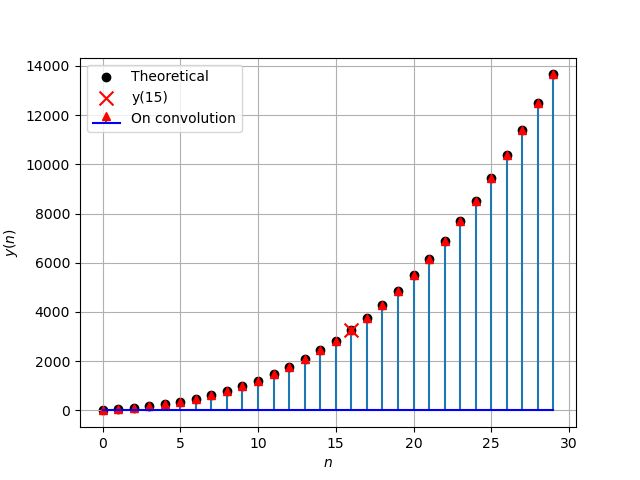
\includegraphics[width=\columnwidth]{ncert-maths/11/9/4/5/figs/plot.png}

\begin{center}
    \caption{Simulation v/s theoretical}
\end{center}
\end{figure}




\item 
Which term of the following sequences:\\
(a) 2,$2\sqrt{2}$,4\dots is 128
\quad(b) $\sqrt{3}$,3,$3\sqrt{3}$\dots is 729\\
(c) $\frac{1}{3}$,$\frac{1}{9}$,$\frac{1}{27}$\dots is $\frac{1}{19683}$ \\
\solution
 \iffalse
\let\negmedspace\undefined
\let\negthickspace\undefined
\documentclass[journal,12pt,twocolumn]{IEEEtran}
\usepackage{amssymb}
\usepackage{cite}
\usepackage{amsmath,amssymb,amsfonts,amsthm}
\usepackage{algorithmic}
\usepackage{graphicx}
\usepackage{textcomp}
\usepackage{xcolor}
\usepackage{txfonts}
\usepackage{listings}
\usepackage{enumitem}
\usepackage{mathtools}
\usepackage{gensymb}
\usepackage{comment}
\usepackage[breaklinks=true]{hyperref}
\usepackage{tkz-euclide} 
\usepackage{listings}
\usepackage{gvv}                                        
\def\inputGnumericTable{}                                 
\usepackage[latin1]{inputenc}                                
\usepackage{color}                                            
\usepackage{array}                                            
\usepackage{longtable}                                       
\usepackage{calc}                                             
\usepackage{multirow}                                         
\usepackage{hhline}                                           
\usepackage{ifthen}                                           
\usepackage{lscape}
\usepackage{pgfplots}
\newtheorem{theorem}{Theorem}[section]
\newtheorem{problem}{Problem}
\newtheorem{proposition}{Proposition}[section]
\newtheorem{lemma}{Lemma}[section]
\newtheorem{corollary}[theorem]{Corollary}
\newtheorem{example}{Example}[section]
\newtheorem{definition}[problem]{Definition}
\newcommand{\BEQA}{\begin{eqnarray}}
\newcommand{\EEQA}{\end{eqnarray}}
\newcommand{\define}{\stackrel{\triangle}{=}}
\theoremstyle{remark}
\newtheorem{rem}{Remark}
\begin{document}

\bibliographystyle{IEEEtran}
\vspace{3cm}

\title{NCERT Discrete-11.9.4-5}
\author{EE22BTECH11004 - Allu Lohith}

\maketitle
\newpage
\bigskip


 Find the sum of n terms of this sequence:$$5^2+6^2+7^2...+20^2$$  
\solution
\fi
\begin{table}[h!]
\centering
\renewcommand{\arraystretch}{2}
\begin{tabular}{|c|p{4cm}|c|}
\hline 
\setlength{\tabcolsep}{1pt}
\textbf{Parameter}  &\textbf{Description} &\textbf{Formulae/Value} \\
\hline
n & Iteration number starting from zero till 15 & - \\
\hline
$x\brak n$ & General term of the sequence from $n=0$ to $n=15$ &$\brak{n+5}^2$  u\brak n\\
\hline
$x\brak 0$ & First term of the sequence & 5 \\
\hline
\end{tabular}

\vspace{0.5cm}
\caption{\normalsize Parameters}
\end{table}
The standard $z$ transforms,
\begin{align}
    u \brak n &\stackrel{z}{\longleftrightarrow} \frac{1}{1-z^{-1}}, \abs z >1\\
   n u\brak n &\stackrel{z}{\longleftrightarrow} \frac{z^{-1}}{\brak{1-z^{-1}}^2}, \abs z >1\\
   n^2 u\brak n &\stackrel{z}{\longleftrightarrow} \frac{z^{-1}\brak{1+z^{-1}}}{\brak{1-z^{-1}}^3}, \abs z >1
\end{align}
As 
\begin{align}
    x\brak n = \brak{n^2+10n+25}u\brak n
\end{align}
The $z$ transform of general term can be written as , 
\begin{align}
    X\brak z &= \frac{z^{-1}\brak{1+z^{-1}}}{\brak{1-z^{-1}}^3}+10\frac{z^{-1}}{\brak{1-z^{-1}}^2}+\frac{25}{1-z^{-1}} \\
    X\brak z &=  \frac{16z^{-2}-39z^{-1}+25}{\brak{1-z^{-1}}^3}; \abs{z}>1
\end{align}
On convolution for finding the sum
\begin{align}
    y\brak n= x\brak n \ast u\brak n
\end{align}
On z transform,
\begin{align}
    Y\brak z &= X \brak z \cdot U \brak z\\
    &= \brak{\frac{16z^{-2}-39z^{-1}+25}{\brak{1-z^{-1}})^3}} \cdot \frac{1}{1-z^{-1}}\\
    \implies 
    Y \brak z & = \frac{16z^{-2}-39z^{-1}+25}{\brak{1-z^{-1}}^4}; \quad \abs z >1
\end{align}
Using the contour integration to find the inverse $z$ transform,
\begin{align}
    y(n)&=\oint_c Y(z)\cdot z^{n-1}dz\\
    y(21)&=\oint_c \brak{\frac{16z^{-2}-39z^{-1}+25}{\brak{1-z^{-1}}^4}} z^{14}dz
\end{align}
As there are four poles from observation, so $m=4$
\begin{align}
    y\brak{21} &= \frac{1}{(m-1)!} \lim_{z \to a} \frac{d^{m-1}}{dz^{m-1}}\brak{(z-a)^mf(z)}\\
    &= \frac{1}{3!} \lim_{z \to 1} \frac{d^{3}}{dz^{3}}\brak{(z-1)^4 \frac{\brak{16z^{-2}-39z^{-1}+25}}{(1-z^{-1})^4} z^{14}}\\
    &= \frac{1}{6} \lim_{z \to 1} \frac{d^{3}}{dz^{3}}\brak{\brak{16z^{-2}-39z^{-1}+25}z^{18}}\\
    &= \frac{1}{6} \lim_{z \to 1} \frac{d^{3}}{dz^{3}}\brak{16z^{16}-39z^{17}+25z^{18}}\\
    &= \frac{1}{6}  \brak{16 \times 18 \times 17 \times 16+14 \times 17 \times 16 \times 15 }\\
    \implies y\brak{21}&=2840 
\end{align}
Hence the sum of the terms of the sequence is 2840.

\begin{figure}[h]
    \centering  

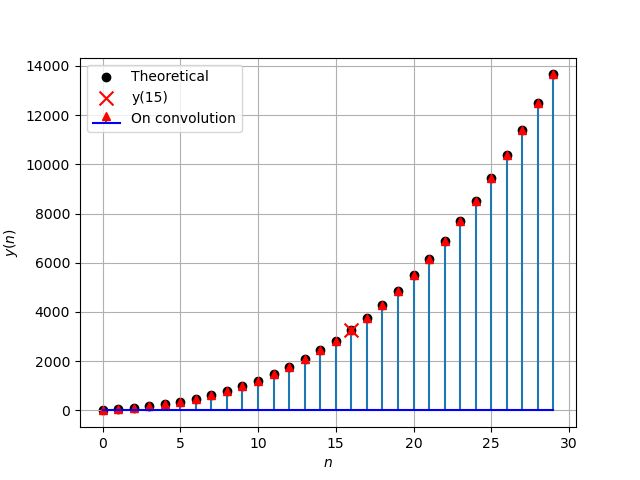
\includegraphics[width=\columnwidth]{ncert-maths/11/9/4/5/figs/plot.png}

\begin{center}
    \caption{Simulation v/s theoretical}
\end{center}
\end{figure}


\clearpage

\item The number of bacteria in a certain culture doubles every hour. If there were 30 bacteria present in the culture originally, how many bacteria will be present at the end of $2^{nd}$ hour, $4^{th}$ hour and $n^{th}$ hour?

\solution
 \iffalse
\let\negmedspace\undefined
\let\negthickspace\undefined
\documentclass[journal,12pt,twocolumn]{IEEEtran}
\usepackage{amssymb}
\usepackage{cite}
\usepackage{amsmath,amssymb,amsfonts,amsthm}
\usepackage{algorithmic}
\usepackage{graphicx}
\usepackage{textcomp}
\usepackage{xcolor}
\usepackage{txfonts}
\usepackage{listings}
\usepackage{enumitem}
\usepackage{mathtools}
\usepackage{gensymb}
\usepackage{comment}
\usepackage[breaklinks=true]{hyperref}
\usepackage{tkz-euclide} 
\usepackage{listings}
\usepackage{gvv}                                        
\def\inputGnumericTable{}                                 
\usepackage[latin1]{inputenc}                                
\usepackage{color}                                            
\usepackage{array}                                            
\usepackage{longtable}                                       
\usepackage{calc}                                             
\usepackage{multirow}                                         
\usepackage{hhline}                                           
\usepackage{ifthen}                                           
\usepackage{lscape}
\usepackage{pgfplots}
\newtheorem{theorem}{Theorem}[section]
\newtheorem{problem}{Problem}
\newtheorem{proposition}{Proposition}[section]
\newtheorem{lemma}{Lemma}[section]
\newtheorem{corollary}[theorem]{Corollary}
\newtheorem{example}{Example}[section]
\newtheorem{definition}[problem]{Definition}
\newcommand{\BEQA}{\begin{eqnarray}}
\newcommand{\EEQA}{\end{eqnarray}}
\newcommand{\define}{\stackrel{\triangle}{=}}
\theoremstyle{remark}
\newtheorem{rem}{Remark}
\begin{document}

\bibliographystyle{IEEEtran}
\vspace{3cm}

\title{NCERT Discrete-11.9.4-5}
\author{EE22BTECH11004 - Allu Lohith}

\maketitle
\newpage
\bigskip


 Find the sum of n terms of this sequence:$$5^2+6^2+7^2...+20^2$$  
\solution
\fi
\begin{table}[h!]
\centering
\renewcommand{\arraystretch}{2}
\begin{tabular}{|c|p{4cm}|c|}
\hline 
\setlength{\tabcolsep}{1pt}
\textbf{Parameter}  &\textbf{Description} &\textbf{Formulae/Value} \\
\hline
n & Iteration number starting from zero till 15 & - \\
\hline
$x\brak n$ & General term of the sequence from $n=0$ to $n=15$ &$\brak{n+5}^2$  u\brak n\\
\hline
$x\brak 0$ & First term of the sequence & 5 \\
\hline
\end{tabular}

\vspace{0.5cm}
\caption{\normalsize Parameters}
\end{table}
The standard $z$ transforms,
\begin{align}
    u \brak n &\stackrel{z}{\longleftrightarrow} \frac{1}{1-z^{-1}}, \abs z >1\\
   n u\brak n &\stackrel{z}{\longleftrightarrow} \frac{z^{-1}}{\brak{1-z^{-1}}^2}, \abs z >1\\
   n^2 u\brak n &\stackrel{z}{\longleftrightarrow} \frac{z^{-1}\brak{1+z^{-1}}}{\brak{1-z^{-1}}^3}, \abs z >1
\end{align}
As 
\begin{align}
    x\brak n = \brak{n^2+10n+25}u\brak n
\end{align}
The $z$ transform of general term can be written as , 
\begin{align}
    X\brak z &= \frac{z^{-1}\brak{1+z^{-1}}}{\brak{1-z^{-1}}^3}+10\frac{z^{-1}}{\brak{1-z^{-1}}^2}+\frac{25}{1-z^{-1}} \\
    X\brak z &=  \frac{16z^{-2}-39z^{-1}+25}{\brak{1-z^{-1}}^3}; \abs{z}>1
\end{align}
On convolution for finding the sum
\begin{align}
    y\brak n= x\brak n \ast u\brak n
\end{align}
On z transform,
\begin{align}
    Y\brak z &= X \brak z \cdot U \brak z\\
    &= \brak{\frac{16z^{-2}-39z^{-1}+25}{\brak{1-z^{-1}})^3}} \cdot \frac{1}{1-z^{-1}}\\
    \implies 
    Y \brak z & = \frac{16z^{-2}-39z^{-1}+25}{\brak{1-z^{-1}}^4}; \quad \abs z >1
\end{align}
Using the contour integration to find the inverse $z$ transform,
\begin{align}
    y(n)&=\oint_c Y(z)\cdot z^{n-1}dz\\
    y(21)&=\oint_c \brak{\frac{16z^{-2}-39z^{-1}+25}{\brak{1-z^{-1}}^4}} z^{14}dz
\end{align}
As there are four poles from observation, so $m=4$
\begin{align}
    y\brak{21} &= \frac{1}{(m-1)!} \lim_{z \to a} \frac{d^{m-1}}{dz^{m-1}}\brak{(z-a)^mf(z)}\\
    &= \frac{1}{3!} \lim_{z \to 1} \frac{d^{3}}{dz^{3}}\brak{(z-1)^4 \frac{\brak{16z^{-2}-39z^{-1}+25}}{(1-z^{-1})^4} z^{14}}\\
    &= \frac{1}{6} \lim_{z \to 1} \frac{d^{3}}{dz^{3}}\brak{\brak{16z^{-2}-39z^{-1}+25}z^{18}}\\
    &= \frac{1}{6} \lim_{z \to 1} \frac{d^{3}}{dz^{3}}\brak{16z^{16}-39z^{17}+25z^{18}}\\
    &= \frac{1}{6}  \brak{16 \times 18 \times 17 \times 16+14 \times 17 \times 16 \times 15 }\\
    \implies y\brak{21}&=2840 
\end{align}
Hence the sum of the terms of the sequence is 2840.

\begin{figure}[h]
    \centering  

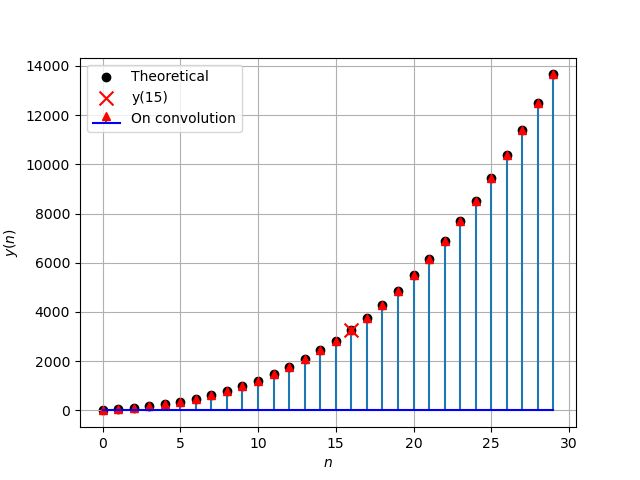
\includegraphics[width=\columnwidth]{ncert-maths/11/9/4/5/figs/plot.png}

\begin{center}
    \caption{Simulation v/s theoretical}
\end{center}
\end{figure}




\item Ramkali saved Rs 5 in the first week of a year and then increased her weekly savings by Rs 1.75. If in the $n$th week, her weekly savings become Rs 20.75, find $n$.

\solution
 \iffalse
\let\negmedspace\undefined
\let\negthickspace\undefined
\documentclass[journal,12pt,twocolumn]{IEEEtran}
\usepackage{amssymb}
\usepackage{cite}
\usepackage{amsmath,amssymb,amsfonts,amsthm}
\usepackage{algorithmic}
\usepackage{graphicx}
\usepackage{textcomp}
\usepackage{xcolor}
\usepackage{txfonts}
\usepackage{listings}
\usepackage{enumitem}
\usepackage{mathtools}
\usepackage{gensymb}
\usepackage{comment}
\usepackage[breaklinks=true]{hyperref}
\usepackage{tkz-euclide} 
\usepackage{listings}
\usepackage{gvv}                                        
\def\inputGnumericTable{}                                 
\usepackage[latin1]{inputenc}                                
\usepackage{color}                                            
\usepackage{array}                                            
\usepackage{longtable}                                       
\usepackage{calc}                                             
\usepackage{multirow}                                         
\usepackage{hhline}                                           
\usepackage{ifthen}                                           
\usepackage{lscape}
\usepackage{pgfplots}
\newtheorem{theorem}{Theorem}[section]
\newtheorem{problem}{Problem}
\newtheorem{proposition}{Proposition}[section]
\newtheorem{lemma}{Lemma}[section]
\newtheorem{corollary}[theorem]{Corollary}
\newtheorem{example}{Example}[section]
\newtheorem{definition}[problem]{Definition}
\newcommand{\BEQA}{\begin{eqnarray}}
\newcommand{\EEQA}{\end{eqnarray}}
\newcommand{\define}{\stackrel{\triangle}{=}}
\theoremstyle{remark}
\newtheorem{rem}{Remark}
\begin{document}

\bibliographystyle{IEEEtran}
\vspace{3cm}

\title{NCERT Discrete-11.9.4-5}
\author{EE22BTECH11004 - Allu Lohith}

\maketitle
\newpage
\bigskip


 Find the sum of n terms of this sequence:$$5^2+6^2+7^2...+20^2$$  
\solution
\fi
\begin{table}[h!]
\centering
\renewcommand{\arraystretch}{2}
\begin{tabular}{|c|p{4cm}|c|}
\hline 
\setlength{\tabcolsep}{1pt}
\textbf{Parameter}  &\textbf{Description} &\textbf{Formulae/Value} \\
\hline
n & Iteration number starting from zero till 15 & - \\
\hline
$x\brak n$ & General term of the sequence from $n=0$ to $n=15$ &$\brak{n+5}^2$  u\brak n\\
\hline
$x\brak 0$ & First term of the sequence & 5 \\
\hline
\end{tabular}

\vspace{0.5cm}
\caption{\normalsize Parameters}
\end{table}
The standard $z$ transforms,
\begin{align}
    u \brak n &\stackrel{z}{\longleftrightarrow} \frac{1}{1-z^{-1}}, \abs z >1\\
   n u\brak n &\stackrel{z}{\longleftrightarrow} \frac{z^{-1}}{\brak{1-z^{-1}}^2}, \abs z >1\\
   n^2 u\brak n &\stackrel{z}{\longleftrightarrow} \frac{z^{-1}\brak{1+z^{-1}}}{\brak{1-z^{-1}}^3}, \abs z >1
\end{align}
As 
\begin{align}
    x\brak n = \brak{n^2+10n+25}u\brak n
\end{align}
The $z$ transform of general term can be written as , 
\begin{align}
    X\brak z &= \frac{z^{-1}\brak{1+z^{-1}}}{\brak{1-z^{-1}}^3}+10\frac{z^{-1}}{\brak{1-z^{-1}}^2}+\frac{25}{1-z^{-1}} \\
    X\brak z &=  \frac{16z^{-2}-39z^{-1}+25}{\brak{1-z^{-1}}^3}; \abs{z}>1
\end{align}
On convolution for finding the sum
\begin{align}
    y\brak n= x\brak n \ast u\brak n
\end{align}
On z transform,
\begin{align}
    Y\brak z &= X \brak z \cdot U \brak z\\
    &= \brak{\frac{16z^{-2}-39z^{-1}+25}{\brak{1-z^{-1}})^3}} \cdot \frac{1}{1-z^{-1}}\\
    \implies 
    Y \brak z & = \frac{16z^{-2}-39z^{-1}+25}{\brak{1-z^{-1}}^4}; \quad \abs z >1
\end{align}
Using the contour integration to find the inverse $z$ transform,
\begin{align}
    y(n)&=\oint_c Y(z)\cdot z^{n-1}dz\\
    y(21)&=\oint_c \brak{\frac{16z^{-2}-39z^{-1}+25}{\brak{1-z^{-1}}^4}} z^{14}dz
\end{align}
As there are four poles from observation, so $m=4$
\begin{align}
    y\brak{21} &= \frac{1}{(m-1)!} \lim_{z \to a} \frac{d^{m-1}}{dz^{m-1}}\brak{(z-a)^mf(z)}\\
    &= \frac{1}{3!} \lim_{z \to 1} \frac{d^{3}}{dz^{3}}\brak{(z-1)^4 \frac{\brak{16z^{-2}-39z^{-1}+25}}{(1-z^{-1})^4} z^{14}}\\
    &= \frac{1}{6} \lim_{z \to 1} \frac{d^{3}}{dz^{3}}\brak{\brak{16z^{-2}-39z^{-1}+25}z^{18}}\\
    &= \frac{1}{6} \lim_{z \to 1} \frac{d^{3}}{dz^{3}}\brak{16z^{16}-39z^{17}+25z^{18}}\\
    &= \frac{1}{6}  \brak{16 \times 18 \times 17 \times 16+14 \times 17 \times 16 \times 15 }\\
    \implies y\brak{21}&=2840 
\end{align}
Hence the sum of the terms of the sequence is 2840.

\begin{figure}[h]
    \centering  

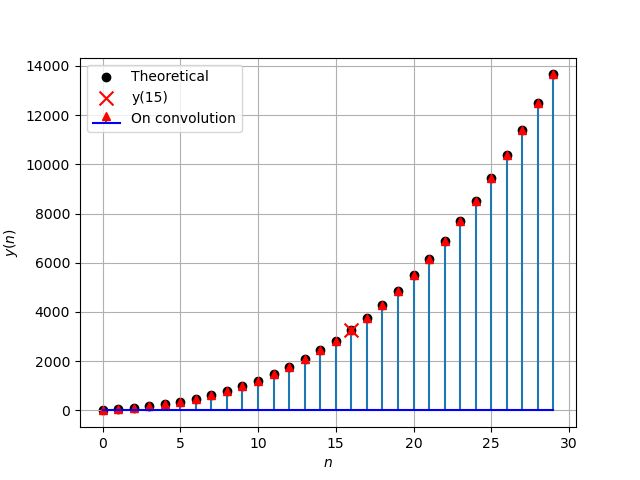
\includegraphics[width=\columnwidth]{ncert-maths/11/9/4/5/figs/plot.png}

\begin{center}
    \caption{Simulation v/s theoretical}
\end{center}
\end{figure}




\item Show that the sum of $\brak {m+n}^{th}$ and $\brak {m-n}^{th}$ terms of an $A.P.,$ is equal to twice the $m^{th}$ terms.    \\
\solution
\input{ncert-maths/11/9/5/1/assignment13.tex}


\item The sum of the first three terms of a G.P is $39/10$ and their product is $1$. Find the common ratio and the terms.\\
\solution
\input{ncert-maths/11/9/3/12/app.tex}


\item The ratio of the A.M and G.M of two positive numbers $a$ and $b$ is $m:n$. Show that $a:b = \brak{ m + \sqrt{m^2 - n^2}} : \brak{ m - \sqrt{m^2 - n^2}}$.\\
\solution
\input{ncert-maths/11/9/5/19/file2.tex}

\item The sum of three numbers in an arithmetic progression (AP) is $24$ and the product of those three numbers is $440$, find the values of the three numbers.\\
\solution
\input{ncert-maths/11/5/9/2/2.tex}
\pagebreak

\item The sum of some terms of G.P. is $315$ whose first term and the common ratio are $5$ and $2$ , respectively. Find the last term and the number of terms.\\
\solution
\input{ncert-maths/11/9/5/8/discrete1.tex}
\pagebreak

\item  Find the sum of n terms of the A.P. whose kth term is \(5k + 1\).\\
\solution
\input{ncert-maths/11/9/2/7/7.tex}
\pagebreak

\item How many 3 digit numbers are divisible by 7? \\
\solution
\input{ncert-maths/10/5/2/13/10.5.2.13.tex}

\item A person writes a letter to four of his friends. He asks each one of them to copy the letter and mail to four different persons with instruction that they move the chain similarly. Assuming that the chain is not broken and that it costs 50 paise to mail one letter. Find the amount spent on the postage when 8th set of letter is mailed.\\
\solution
\input{ncert-maths/11/9/5/29/first.tex}
\pagebreak

\item If $a$, $b$, $c$ are in A.P.; $b$, $c$, $d$ are in G.P and $\frac{1}{c}$, $\frac{1}{d}$, $\frac{1}{e}$ are in A.P. prove that $a$, $c$, $e$ are in G.P.\\
\solution
\input{ncert-maths/11/9/5/20/20.tex}
\pagebreak

\item Find the 31st term of an AP whose $11$th term is 38 and the $16$th term is 73.\\ 
\solution
 \iffalse
\let\negmedspace\undefined
\let\negthickspace\undefined
\documentclass[journal,12pt,twocolumn]{IEEEtran}
\usepackage{amssymb}
\usepackage{cite}
\usepackage{amsmath,amssymb,amsfonts,amsthm}
\usepackage{algorithmic}
\usepackage{graphicx}
\usepackage{textcomp}
\usepackage{xcolor}
\usepackage{txfonts}
\usepackage{listings}
\usepackage{enumitem}
\usepackage{mathtools}
\usepackage{gensymb}
\usepackage{comment}
\usepackage[breaklinks=true]{hyperref}
\usepackage{tkz-euclide} 
\usepackage{listings}
\usepackage{gvv}                                        
\def\inputGnumericTable{}                                 
\usepackage[latin1]{inputenc}                                
\usepackage{color}                                            
\usepackage{array}                                            
\usepackage{longtable}                                       
\usepackage{calc}                                             
\usepackage{multirow}                                         
\usepackage{hhline}                                           
\usepackage{ifthen}                                           
\usepackage{lscape}
\usepackage{pgfplots}
\newtheorem{theorem}{Theorem}[section]
\newtheorem{problem}{Problem}
\newtheorem{proposition}{Proposition}[section]
\newtheorem{lemma}{Lemma}[section]
\newtheorem{corollary}[theorem]{Corollary}
\newtheorem{example}{Example}[section]
\newtheorem{definition}[problem]{Definition}
\newcommand{\BEQA}{\begin{eqnarray}}
\newcommand{\EEQA}{\end{eqnarray}}
\newcommand{\define}{\stackrel{\triangle}{=}}
\theoremstyle{remark}
\newtheorem{rem}{Remark}
\begin{document}

\bibliographystyle{IEEEtran}
\vspace{3cm}

\title{NCERT Discrete-11.9.4-5}
\author{EE22BTECH11004 - Allu Lohith}

\maketitle
\newpage
\bigskip


 Find the sum of n terms of this sequence:$$5^2+6^2+7^2...+20^2$$  
\solution
\fi
\begin{table}[h!]
\centering
\renewcommand{\arraystretch}{2}
\begin{tabular}{|c|p{4cm}|c|}
\hline 
\setlength{\tabcolsep}{1pt}
\textbf{Parameter}  &\textbf{Description} &\textbf{Formulae/Value} \\
\hline
n & Iteration number starting from zero till 15 & - \\
\hline
$x\brak n$ & General term of the sequence from $n=0$ to $n=15$ &$\brak{n+5}^2$  u\brak n\\
\hline
$x\brak 0$ & First term of the sequence & 5 \\
\hline
\end{tabular}

\vspace{0.5cm}
\caption{\normalsize Parameters}
\end{table}
The standard $z$ transforms,
\begin{align}
    u \brak n &\stackrel{z}{\longleftrightarrow} \frac{1}{1-z^{-1}}, \abs z >1\\
   n u\brak n &\stackrel{z}{\longleftrightarrow} \frac{z^{-1}}{\brak{1-z^{-1}}^2}, \abs z >1\\
   n^2 u\brak n &\stackrel{z}{\longleftrightarrow} \frac{z^{-1}\brak{1+z^{-1}}}{\brak{1-z^{-1}}^3}, \abs z >1
\end{align}
As 
\begin{align}
    x\brak n = \brak{n^2+10n+25}u\brak n
\end{align}
The $z$ transform of general term can be written as , 
\begin{align}
    X\brak z &= \frac{z^{-1}\brak{1+z^{-1}}}{\brak{1-z^{-1}}^3}+10\frac{z^{-1}}{\brak{1-z^{-1}}^2}+\frac{25}{1-z^{-1}} \\
    X\brak z &=  \frac{16z^{-2}-39z^{-1}+25}{\brak{1-z^{-1}}^3}; \abs{z}>1
\end{align}
On convolution for finding the sum
\begin{align}
    y\brak n= x\brak n \ast u\brak n
\end{align}
On z transform,
\begin{align}
    Y\brak z &= X \brak z \cdot U \brak z\\
    &= \brak{\frac{16z^{-2}-39z^{-1}+25}{\brak{1-z^{-1}})^3}} \cdot \frac{1}{1-z^{-1}}\\
    \implies 
    Y \brak z & = \frac{16z^{-2}-39z^{-1}+25}{\brak{1-z^{-1}}^4}; \quad \abs z >1
\end{align}
Using the contour integration to find the inverse $z$ transform,
\begin{align}
    y(n)&=\oint_c Y(z)\cdot z^{n-1}dz\\
    y(21)&=\oint_c \brak{\frac{16z^{-2}-39z^{-1}+25}{\brak{1-z^{-1}}^4}} z^{14}dz
\end{align}
As there are four poles from observation, so $m=4$
\begin{align}
    y\brak{21} &= \frac{1}{(m-1)!} \lim_{z \to a} \frac{d^{m-1}}{dz^{m-1}}\brak{(z-a)^mf(z)}\\
    &= \frac{1}{3!} \lim_{z \to 1} \frac{d^{3}}{dz^{3}}\brak{(z-1)^4 \frac{\brak{16z^{-2}-39z^{-1}+25}}{(1-z^{-1})^4} z^{14}}\\
    &= \frac{1}{6} \lim_{z \to 1} \frac{d^{3}}{dz^{3}}\brak{\brak{16z^{-2}-39z^{-1}+25}z^{18}}\\
    &= \frac{1}{6} \lim_{z \to 1} \frac{d^{3}}{dz^{3}}\brak{16z^{16}-39z^{17}+25z^{18}}\\
    &= \frac{1}{6}  \brak{16 \times 18 \times 17 \times 16+14 \times 17 \times 16 \times 15 }\\
    \implies y\brak{21}&=2840 
\end{align}
Hence the sum of the terms of the sequence is 2840.

\begin{figure}[h]
    \centering  

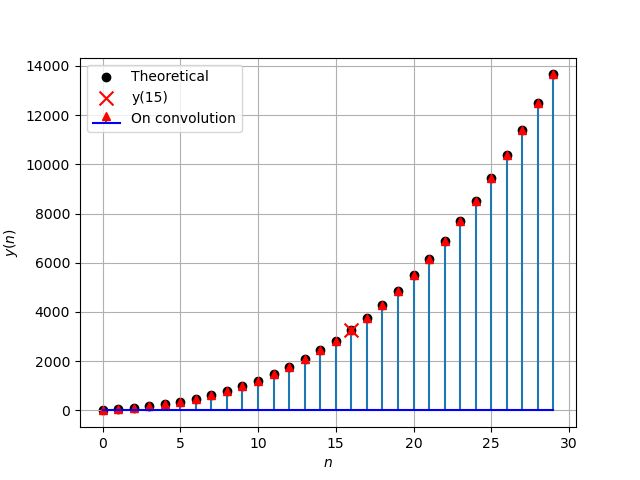
\includegraphics[width=\columnwidth]{ncert-maths/11/9/4/5/figs/plot.png}

\begin{center}
    \caption{Simulation v/s theoretical}
\end{center}
\end{figure}



\pagebreak
\item If $a\left(\frac{1}{b} + \frac{1}{c}\right)$, $b\left(\frac{1}{c} + \frac{1}{a}\right)$, $c\left(\frac{1}{a} + \frac{1}{b}\right)$ are in arithmetic progression (AP), prove that $a$, $b$, $c$ are also in AP. \\
\solution
 \iffalse
\let\negmedspace\undefined
\let\negthickspace\undefined
\documentclass[journal,12pt,twocolumn]{IEEEtran}
\usepackage{amssymb}
\usepackage{cite}
\usepackage{amsmath,amssymb,amsfonts,amsthm}
\usepackage{algorithmic}
\usepackage{graphicx}
\usepackage{textcomp}
\usepackage{xcolor}
\usepackage{txfonts}
\usepackage{listings}
\usepackage{enumitem}
\usepackage{mathtools}
\usepackage{gensymb}
\usepackage{comment}
\usepackage[breaklinks=true]{hyperref}
\usepackage{tkz-euclide} 
\usepackage{listings}
\usepackage{gvv}                                        
\def\inputGnumericTable{}                                 
\usepackage[latin1]{inputenc}                                
\usepackage{color}                                            
\usepackage{array}                                            
\usepackage{longtable}                                       
\usepackage{calc}                                             
\usepackage{multirow}                                         
\usepackage{hhline}                                           
\usepackage{ifthen}                                           
\usepackage{lscape}
\usepackage{pgfplots}
\newtheorem{theorem}{Theorem}[section]
\newtheorem{problem}{Problem}
\newtheorem{proposition}{Proposition}[section]
\newtheorem{lemma}{Lemma}[section]
\newtheorem{corollary}[theorem]{Corollary}
\newtheorem{example}{Example}[section]
\newtheorem{definition}[problem]{Definition}
\newcommand{\BEQA}{\begin{eqnarray}}
\newcommand{\EEQA}{\end{eqnarray}}
\newcommand{\define}{\stackrel{\triangle}{=}}
\theoremstyle{remark}
\newtheorem{rem}{Remark}
\begin{document}

\bibliographystyle{IEEEtran}
\vspace{3cm}

\title{NCERT Discrete-11.9.4-5}
\author{EE22BTECH11004 - Allu Lohith}

\maketitle
\newpage
\bigskip


 Find the sum of n terms of this sequence:$$5^2+6^2+7^2...+20^2$$  
\solution
\fi
\begin{table}[h!]
\centering
\renewcommand{\arraystretch}{2}
\begin{tabular}{|c|p{4cm}|c|}
\hline 
\setlength{\tabcolsep}{1pt}
\textbf{Parameter}  &\textbf{Description} &\textbf{Formulae/Value} \\
\hline
n & Iteration number starting from zero till 15 & - \\
\hline
$x\brak n$ & General term of the sequence from $n=0$ to $n=15$ &$\brak{n+5}^2$  u\brak n\\
\hline
$x\brak 0$ & First term of the sequence & 5 \\
\hline
\end{tabular}

\vspace{0.5cm}
\caption{\normalsize Parameters}
\end{table}
The standard $z$ transforms,
\begin{align}
    u \brak n &\stackrel{z}{\longleftrightarrow} \frac{1}{1-z^{-1}}, \abs z >1\\
   n u\brak n &\stackrel{z}{\longleftrightarrow} \frac{z^{-1}}{\brak{1-z^{-1}}^2}, \abs z >1\\
   n^2 u\brak n &\stackrel{z}{\longleftrightarrow} \frac{z^{-1}\brak{1+z^{-1}}}{\brak{1-z^{-1}}^3}, \abs z >1
\end{align}
As 
\begin{align}
    x\brak n = \brak{n^2+10n+25}u\brak n
\end{align}
The $z$ transform of general term can be written as , 
\begin{align}
    X\brak z &= \frac{z^{-1}\brak{1+z^{-1}}}{\brak{1-z^{-1}}^3}+10\frac{z^{-1}}{\brak{1-z^{-1}}^2}+\frac{25}{1-z^{-1}} \\
    X\brak z &=  \frac{16z^{-2}-39z^{-1}+25}{\brak{1-z^{-1}}^3}; \abs{z}>1
\end{align}
On convolution for finding the sum
\begin{align}
    y\brak n= x\brak n \ast u\brak n
\end{align}
On z transform,
\begin{align}
    Y\brak z &= X \brak z \cdot U \brak z\\
    &= \brak{\frac{16z^{-2}-39z^{-1}+25}{\brak{1-z^{-1}})^3}} \cdot \frac{1}{1-z^{-1}}\\
    \implies 
    Y \brak z & = \frac{16z^{-2}-39z^{-1}+25}{\brak{1-z^{-1}}^4}; \quad \abs z >1
\end{align}
Using the contour integration to find the inverse $z$ transform,
\begin{align}
    y(n)&=\oint_c Y(z)\cdot z^{n-1}dz\\
    y(21)&=\oint_c \brak{\frac{16z^{-2}-39z^{-1}+25}{\brak{1-z^{-1}}^4}} z^{14}dz
\end{align}
As there are four poles from observation, so $m=4$
\begin{align}
    y\brak{21} &= \frac{1}{(m-1)!} \lim_{z \to a} \frac{d^{m-1}}{dz^{m-1}}\brak{(z-a)^mf(z)}\\
    &= \frac{1}{3!} \lim_{z \to 1} \frac{d^{3}}{dz^{3}}\brak{(z-1)^4 \frac{\brak{16z^{-2}-39z^{-1}+25}}{(1-z^{-1})^4} z^{14}}\\
    &= \frac{1}{6} \lim_{z \to 1} \frac{d^{3}}{dz^{3}}\brak{\brak{16z^{-2}-39z^{-1}+25}z^{18}}\\
    &= \frac{1}{6} \lim_{z \to 1} \frac{d^{3}}{dz^{3}}\brak{16z^{16}-39z^{17}+25z^{18}}\\
    &= \frac{1}{6}  \brak{16 \times 18 \times 17 \times 16+14 \times 17 \times 16 \times 15 }\\
    \implies y\brak{21}&=2840 
\end{align}
Hence the sum of the terms of the sequence is 2840.

\begin{figure}[h]
    \centering  

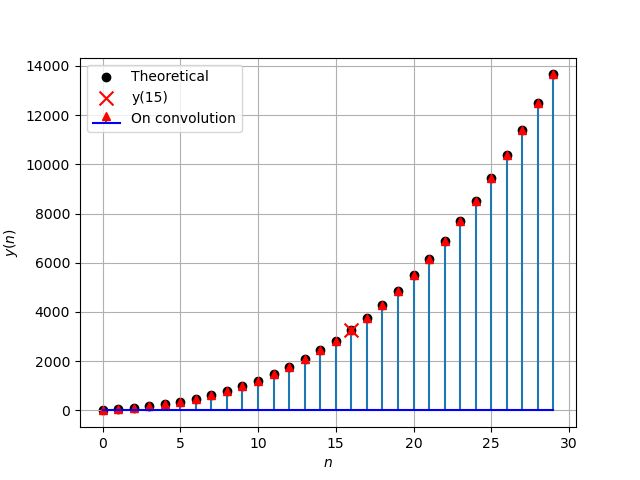
\includegraphics[width=\columnwidth]{ncert-maths/11/9/4/5/figs/plot.png}

\begin{center}
    \caption{Simulation v/s theoretical}
\end{center}
\end{figure}


\newpage
\item If \(\frac{a^n +b^n}{a^{n-1} + b^{n-1}}\) is A.M between $a$ and $b$, then find value of $n$.\\
\solution
\input{ncert-maths/11/9/2/15/discrete[11.9.2.15].tex}
\pagebreak

\item The 17th term of ap exceeds its 10th term by 7. FInd its common difference?\\
 \solution
\input{ncert-maths/10/5/2/11/assignment.tex}
 \pagebreak
 \item If $p^{th},q^{th},r^{th} $ term of a GP are $a,b$ and $c$  respectively Prove that \\
\begin{align*}
    a^{q-r}b^{r-p}c^{p-q}=1
\end{align*}
\solution
\input{ncert-maths/11/9/3/22/assignment4.tex}
\pagebreak

\item Write the first five terms of the sequence whose $n^{th}$ \text{term is} : $x(n) = (-1)^{n-1}5^{n+1}$.\\
\solution
 \iffalse
\let\negmedspace\undefined
\let\negthickspace\undefined
\documentclass[journal,12pt,twocolumn]{IEEEtran}
\usepackage{amssymb}
\usepackage{cite}
\usepackage{amsmath,amssymb,amsfonts,amsthm}
\usepackage{algorithmic}
\usepackage{graphicx}
\usepackage{textcomp}
\usepackage{xcolor}
\usepackage{txfonts}
\usepackage{listings}
\usepackage{enumitem}
\usepackage{mathtools}
\usepackage{gensymb}
\usepackage{comment}
\usepackage[breaklinks=true]{hyperref}
\usepackage{tkz-euclide} 
\usepackage{listings}
\usepackage{gvv}                                        
\def\inputGnumericTable{}                                 
\usepackage[latin1]{inputenc}                                
\usepackage{color}                                            
\usepackage{array}                                            
\usepackage{longtable}                                       
\usepackage{calc}                                             
\usepackage{multirow}                                         
\usepackage{hhline}                                           
\usepackage{ifthen}                                           
\usepackage{lscape}
\usepackage{pgfplots}
\newtheorem{theorem}{Theorem}[section]
\newtheorem{problem}{Problem}
\newtheorem{proposition}{Proposition}[section]
\newtheorem{lemma}{Lemma}[section]
\newtheorem{corollary}[theorem]{Corollary}
\newtheorem{example}{Example}[section]
\newtheorem{definition}[problem]{Definition}
\newcommand{\BEQA}{\begin{eqnarray}}
\newcommand{\EEQA}{\end{eqnarray}}
\newcommand{\define}{\stackrel{\triangle}{=}}
\theoremstyle{remark}
\newtheorem{rem}{Remark}
\begin{document}

\bibliographystyle{IEEEtran}
\vspace{3cm}

\title{NCERT Discrete-11.9.4-5}
\author{EE22BTECH11004 - Allu Lohith}

\maketitle
\newpage
\bigskip


 Find the sum of n terms of this sequence:$$5^2+6^2+7^2...+20^2$$  
\solution
\fi
\begin{table}[h!]
\centering
\renewcommand{\arraystretch}{2}
\begin{tabular}{|c|p{4cm}|c|}
\hline 
\setlength{\tabcolsep}{1pt}
\textbf{Parameter}  &\textbf{Description} &\textbf{Formulae/Value} \\
\hline
n & Iteration number starting from zero till 15 & - \\
\hline
$x\brak n$ & General term of the sequence from $n=0$ to $n=15$ &$\brak{n+5}^2$  u\brak n\\
\hline
$x\brak 0$ & First term of the sequence & 5 \\
\hline
\end{tabular}

\vspace{0.5cm}
\caption{\normalsize Parameters}
\end{table}
The standard $z$ transforms,
\begin{align}
    u \brak n &\stackrel{z}{\longleftrightarrow} \frac{1}{1-z^{-1}}, \abs z >1\\
   n u\brak n &\stackrel{z}{\longleftrightarrow} \frac{z^{-1}}{\brak{1-z^{-1}}^2}, \abs z >1\\
   n^2 u\brak n &\stackrel{z}{\longleftrightarrow} \frac{z^{-1}\brak{1+z^{-1}}}{\brak{1-z^{-1}}^3}, \abs z >1
\end{align}
As 
\begin{align}
    x\brak n = \brak{n^2+10n+25}u\brak n
\end{align}
The $z$ transform of general term can be written as , 
\begin{align}
    X\brak z &= \frac{z^{-1}\brak{1+z^{-1}}}{\brak{1-z^{-1}}^3}+10\frac{z^{-1}}{\brak{1-z^{-1}}^2}+\frac{25}{1-z^{-1}} \\
    X\brak z &=  \frac{16z^{-2}-39z^{-1}+25}{\brak{1-z^{-1}}^3}; \abs{z}>1
\end{align}
On convolution for finding the sum
\begin{align}
    y\brak n= x\brak n \ast u\brak n
\end{align}
On z transform,
\begin{align}
    Y\brak z &= X \brak z \cdot U \brak z\\
    &= \brak{\frac{16z^{-2}-39z^{-1}+25}{\brak{1-z^{-1}})^3}} \cdot \frac{1}{1-z^{-1}}\\
    \implies 
    Y \brak z & = \frac{16z^{-2}-39z^{-1}+25}{\brak{1-z^{-1}}^4}; \quad \abs z >1
\end{align}
Using the contour integration to find the inverse $z$ transform,
\begin{align}
    y(n)&=\oint_c Y(z)\cdot z^{n-1}dz\\
    y(21)&=\oint_c \brak{\frac{16z^{-2}-39z^{-1}+25}{\brak{1-z^{-1}}^4}} z^{14}dz
\end{align}
As there are four poles from observation, so $m=4$
\begin{align}
    y\brak{21} &= \frac{1}{(m-1)!} \lim_{z \to a} \frac{d^{m-1}}{dz^{m-1}}\brak{(z-a)^mf(z)}\\
    &= \frac{1}{3!} \lim_{z \to 1} \frac{d^{3}}{dz^{3}}\brak{(z-1)^4 \frac{\brak{16z^{-2}-39z^{-1}+25}}{(1-z^{-1})^4} z^{14}}\\
    &= \frac{1}{6} \lim_{z \to 1} \frac{d^{3}}{dz^{3}}\brak{\brak{16z^{-2}-39z^{-1}+25}z^{18}}\\
    &= \frac{1}{6} \lim_{z \to 1} \frac{d^{3}}{dz^{3}}\brak{16z^{16}-39z^{17}+25z^{18}}\\
    &= \frac{1}{6}  \brak{16 \times 18 \times 17 \times 16+14 \times 17 \times 16 \times 15 }\\
    \implies y\brak{21}&=2840 
\end{align}
Hence the sum of the terms of the sequence is 2840.

\begin{figure}[h]
    \centering  

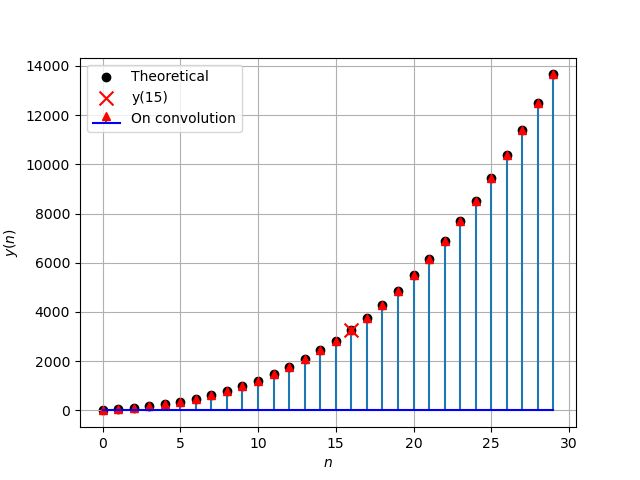
\includegraphics[width=\columnwidth]{ncert-maths/11/9/4/5/figs/plot.png}

\begin{center}
    \caption{Simulation v/s theoretical}
\end{center}
\end{figure}


\pagebreak
\item The ratio of sums of m and n terms of an A.P. is $m^2:n^2$.Show
that the ratio of $m^{th}$ and $n^{th}$ term is (2m-1):(2n-1).\\
\solution
\pagebreak

\item If $a$ and $b$ are the roots of $x^{2} -3x + p = 0$ and $c$ , $d$ are roots of $x^{2} - 12x + q = 0$ where $a,b,c,d$ form a G.P. Prove that $(q+p) : (q-p)$ = 17:15 .\\
\solution
\pagebreak


\item Write the first five terms in the sequence defined recursively as follows:
\[ a_{0} = 3 \]
\[ a_{n} = 3a_{n-1} + 2 \quad \text{for } n > 0 \]
\solution 
\pagebreak


\item \begin{align}
\frac{a+bx}{a-bx}=\frac{b+cx}{b-cx}=\frac{c+dx}{c-dx}
\end{align}
then show that a,b,c,d are in G.P\\
\solution
\input{ncert-maths/11/9/5/13/assign2.tex}
\pagebreak


\item Sum of the first p, q and r terms of an A.P. are a, b and c, respectively.\\
Prove that $\dfrac{a}{p}\brak{q-r}+\dfrac{b}{q}\brak{r-p}+\dfrac{c}{r}\brak{p-q}=0$\hfill{NCERT-discrete 11.9.2.11}\\
\solution
\iffalse
\documentclass[journal,12pt,twocolumn]{IEEEtran}
\usepackage{cite}
\usepackage{amsmath,amssymb,amsfonts,amsthm,mathtools}
\usepackage{algorithmic}
\usepackage{graphicx}
\parindent 0px
\bibliographystyle{IEEEtran}
\title{NCERT DISCRETE 11.9.2 Q10}
\author{EE23BTECH11052 - Abhilash Rapolu }
\begin{document}
\maketitle
\newpage
\textbf{Question 11.9.2.10}:If the sum of first $p$ terms of an A.P. is equal to the sum of the first $q$ terms, then
find the sum of the first $(p + q)$ terms.\\
\ Solution:
\fi
\begin{table}[htbp]
\centering
\begin{tabular}{|l|l|c|}
\hline
\textbf{Parameter} & \textbf{Description} & \textbf{Value} \\
\hline
$a_0$ & first term & none \\
\hline
$d$ & common difference & none \\
\hline
$x(n)$ & $n^{th}$ term & $a_0+nd$ \\
\hline
$y(n)$ & Sum of n terms  & $\frac{n+1}{2}[2a_0+nd]$ \\
\hline
$y(p-1)$ & sum of first p terms & $\frac{p}{2}[2a_0+(p-1)d]$ \\
\hline
$y(q-1)$ & sum of first q terms & $\frac{q}{2}[2a_0+(q-1)d]$ \\
\hline
$y(p+q-1)$ & sum of first p+q terms & $\frac{p+q}{2}[2a_0+(p+q-1)d]$ \\
\hline
\end{tabular}


\caption{Given parameters list}
\end{table}
Now let's find the z transform of the $x(n)$ using the linearity property.\\
\begin{align}
X(z)&=\frac{a_0}{1-z^{-1}}+d\frac{z^{-1}}{(1-z^{-1})^2}\\
y(n) &= x(n)*u(n)
\end{align}
Now apply z transform on both sides\\
\begin{align}
Y(z)&=X(z)U(z)\\
Y(z)&=\frac{a_0}{(1-z^{-1})^2}+d\frac{z^{-1}}{(1-z^{-1})^3}
\end{align}
by comparison of the above equations:\\
using equations from appendix  \eqref{eq:uzder-shift} and \eqref{eq:uzder-der}\\
the inverse z transform:\\
\begin{align}
y(n)&=[a_0(n)+\frac{d}{2}(n)(n-1)]u(n)
\end{align}
as we considered n=0 as our first term, we have to replace n by (n+1)\\
Sum of first n terms is given as:\\
\begin{align}
y(n)&=[a_0(n+1)+\frac{d}{2}(n+1)(n)]u(n)
\end{align}
given in question y(p-1)=y(q-1)\\
\begin{align}
[a_0(p)+\frac{d}{2}(p-1)(p)]u(n)&=[a_0(q)+\frac{d}{2}(q-1)(q)]u(n)\\
d&=(-)\frac{2a_0}{p+q-1}
\end{align}
now for first p+q terms:\\
\begin{align}
y(p+q-1)&=[a_0(p+q)+\frac{d}{2}(p+q-1)(p+q)]u(n)
\end{align}
substitue d in this\\
\begin{align}
y(p+q-1)&=[a_0(p+q)-\frac{a_0}{p+q-1}(p+q-1)(p+q)]u(n)\\
y(p+q-1)&=[a_0(p+q)-a_0(p+q)]u(n)\\
y(p+q-1)&=0.
\end{align}

%\end{document}


\pagebreak

\item The pth, qth and rth terms of an AP are a,b,c respectively. Show that
\begin{align*} (q-r)a + (r-p)b +(p-q)c =0 \end{align*}
\solution
\input{ncert-maths/11/9/5/15/11.9.5.15.tex}
\pagebreak

\item Find the sum to indicated number of term in each of the geometric progressions in $\sqrt{7} ,\sqrt{21} , 3\sqrt{7}, ....n$ terms\\
\solution
\input{ncert-maths/11/9/3/8/8.tex}

\item How many multiples of 4 lie between 10 and 250?\\
\solution
\iffalse
\let\negmedspace\undefined
\let\negthickspace\undefined
\documentclass[journal,12pt,twocolumn]{IEEEtran}
\usepackage{cite}
\usepackage{amsmath,amssymb,amsfonts,amsthm}
\usepackage{algorithmic}
\usepackage{graphicx}
\usepackage{textcomp}
\usepackage{xcolor}
\usepackage{txfonts}
\usepackage{listings}
\usepackage{enumitem}
\usepackage{mathtools}
\usepackage{gensymb}
\usepackage{comment}
\usepackage[breaklinks=true]{hyperref}
\usepackage{tkz-euclide} 
\usepackage{listings}
\usepackage{gvv}                                        
\def\inputGnumericTable{}                                 
\usepackage[latin1]{inputenc}                                
\usepackage{color}                                            
\usepackage{array}                                            
\usepackage{longtable}                                       
\usepackage{calc}                                             
\usepackage{multirow}                                         
\usepackage{hhline}                                           
\usepackage{ifthen}                                           
\usepackage{lscape}
\usepackage{caption}
\newtheorem{theorem}{Theorem}[section]
\newtheorem{problem}{Problem}
\newtheorem{proposition}{Proposition}[section]
\newtheorem{lemma}{Lemma}[section]
\newtheorem{corollary}[theorem]{Corollary}
\newtheorem{example}{Example}[section]
\newtheorem{definition}[problem]{Definition}
\newcommand{\BEQA}{\begin{eqnarray}}
\newcommand{\EEQA}{\end{eqnarray}}
\newcommand{\define}{\stackrel{\triangle}{=}}
\theoremstyle{remark}
\newtheorem{rem}{Remark}
\begin{document}

\bibliographystyle{IEEEtran}
\vspace{3cm}

\title{10.5.2.14}
\author{EE23BTECH11003 - pranav}
\maketitle
\newpage

\bigskip
\renewcommand{\thefigure}{\arabic{figure}}
\renewcommand{\thetable}{\arabic{table}}

\textbf{Question}:
How many multiples of 4 lie between 10 and 250?\\
\solution
\fi
\begin{table}[h]
    \centering
    \input{ncert-maths/10/5/2/14/tables/Table.Tex}
    \caption{Variables Used}
    \label{tab:10.5.2.14}
\end{table}
\begin{align}
    n&=\frac{(250-250 \text{ mod } 2)-(10+10\text{ mod } 2)}{4}+1\\
    n&=60
\end{align}
Considering the series to start from $n=0$,the general term is
\begin{align}
x(n)&=(x(0)+nd)u(n)\\
x(n)&=(12+4n)u(n)
\end{align}
\begin{figure}[h!]
    \centering
    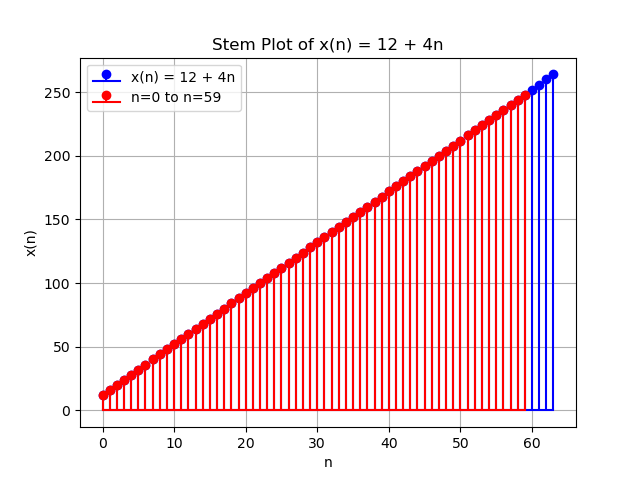
\includegraphics[width=\linewidth]{ncert-maths/10/5/2/14/figs/graph1.png}
    \caption{stem plot of x(n)}
\end{figure}
applying Z transform
\begin{align}
    X(z)&= \sum_{n=-\infty}^{\infty}x(n) z^{-n}\\
   \implies X(z)&= \sum_{n=-\infty}^{\infty} (12+4n) u(n) z^{-n}\\
   \implies X(z) &=\sum_{n= 0}^{\infty} (12+4n)  z^{-n}\\
   \implies X(z)&=\frac{12}{1-z^{-1}}+\frac{4 z^{-1}}{(1-z^{-1})^{2}}\quad \abs{z}>1
\end{align}
%\end{document}

\pagebreak

\item if $a,b,c$ and $d$ are in GP then show that $(a^{2}+b^{2}+c^{2})(b^{2}+c^{2}+d^{2})=(ab+bc+cd)^{2}$\\
\solution
\pagebreak

\item In an A.P. the first term is 2 and the sum of the first five terms is one-fourth of the next five terms. Show that 20\textsuperscript{th} term is $-112$. \hfill(NCERT MATHS 11.9.2.3)\\
\solution
\input{ncert-maths/11/9/2/3/a_0.tex}
\pagebreak
\item If the 3rd and the 9th terms of an AP are 4 and -8, respectively, which term of this AP is zero? \\
\solution
\pagebreak
\item Find the sum of the products of the corresponding terms of the sequences $2, 4, 8, 16, 32$ and $128, 32, 8, 2, \frac{1}{2}$.
\solution
\pagebreak

\item Let the sum of $n,2n,3n$ terms of an AP be $S_1,S_2$ and $S_3$, respectively, show that $S_3=3(S_2-S_1)$\\
\solution
\iffalse
\let\negthickspace\undefined
\documentclass[journal,12pt,twocolumn]{IEEEtran}
\usepackage{cite}
\usepackage{amsmath,amssymb,amsfonts,amsthm}
\usepackage{algorithmic}
\usepackage{graphicx}
\usepackage{textcomp}
\usepackage{xcolor}
\usepackage{txfonts}
\usepackage{listings}
\usepackage{enumitem}
\usepackage{mathtools}
\usepackage{gensymb}
\usepackage{comment}
\usepackage[breaklinks=true]{hyperref}
\usepackage{tkz-euclide} 
\usepackage{listings}
\usepackage{gvv}                                        
\def\inputGnumericTable{}                                 
\usepackage[latin1]{inputenc}                                
\usepackage{color}                                            
\usepackage{array}                                            
\usepackage{longtable}                                       
\usepackage{calc}                                             
\usepackage{multirow}                                         
\usepackage{hhline}                                           
\usepackage{ifthen}                                           
\usepackage{lscape}
\usepackage{tfrupee}

\newtheorem{theorem}{Theorem}[section]
\newtheorem{problem}{Problem}
\newtheorem{proposition}{Proposition}[section]
\newtheorem{lemma}{Lemma}[section]
\newtheorem{corollary}[theorem]{Corollary}
\newtheorem{example}{Example}[section]
\newtheorem{definition}[problem]{Definition}
\newcommand{\BEQA}{\begin{eqnarray}}
\newcommand{\EEQA}{\end{eqnarray}}
\newcommand{\define}{\stackrel{\triangle}{=}}
\theoremstyle{remark}
\newtheorem{rem}{Remark}
\begin{document}

\bibliographystyle{IEEEtran}
\vspace{3cm}

\title{11.9.5.3}
\author{EE23BTECH11062 - V MANAS}
\maketitle
\newpage

\bigskip
\textbf{Question:}\\Let the sum of $n,2n,3n$ terms of an AP be $S_1,S_2$ and $S_3$, respectively, show that $S_3=3(S_2-S_1)$\\
\textbf{Solution:}
\fi
\begin{table}[h]
    \centering
    \begin{tabular}{|c|c|c|}
    \hline
    \textbf{Variable} & \textbf{Description}\\
    \hline
    x(0) & First term of AP\\
    \hline
    d & common difference in the AP\\
    \hline
    n & number of terms in AP\\
    \hline
    y(n) & sum of n terms of the AP\\
    \hline
\end{tabular}

    \caption{Variables Used}
    \label{tab:table_11.9.5.3}
\end{table}
\begin{figure}[h]
    \centering
    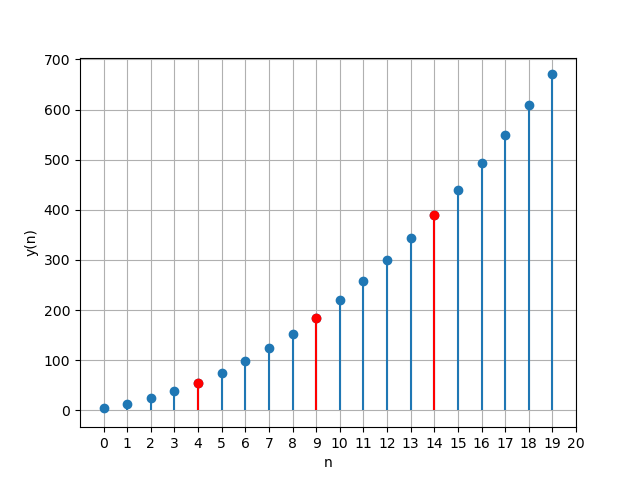
\includegraphics[width=\linewidth]{ncert-maths/11/9/5/3/figs/graph.png}
    \caption{Verification plot for the AP[y(n)=$\frac{n+1}{2}(2(5)+n(3))u(n)$]}
\end{figure}\\
By equation(\ref{eq:3/ap/contour})
\begin{align}
    y(n)&=\frac{n+1}{2}(2x(0)+nd)u(n)\\
    y(2n)&=\frac{2n+1}{2}(2x(0)+2nd)u(n)\\
    y(3n)&=\frac{3n+1}{2}(2x(0)+3nd)u(n)\\
    3(y(2n)-y(n))&=\frac{3n+1}{2}(2x(0)+3nd)u(n)
\end{align}

%\end{document}

\pagebreak

\item Show that the products of the corresponding terms of the sequences $a, ar, ar2, \ldots ar^{n-1}$ and $A, AR, AR2, \ldots AR^{n-1}$ form a G.P, and find the common ratio.
\solution
 \iffalse
\let\negmedspace\undefined
\let\negthickspace\undefined
\documentclass[journal,12pt,twocolumn]{IEEEtran}
\usepackage{amssymb}
\usepackage{cite}
\usepackage{amsmath,amssymb,amsfonts,amsthm}
\usepackage{algorithmic}
\usepackage{graphicx}
\usepackage{textcomp}
\usepackage{xcolor}
\usepackage{txfonts}
\usepackage{listings}
\usepackage{enumitem}
\usepackage{mathtools}
\usepackage{gensymb}
\usepackage{comment}
\usepackage[breaklinks=true]{hyperref}
\usepackage{tkz-euclide} 
\usepackage{listings}
\usepackage{gvv}                                        
\def\inputGnumericTable{}                                 
\usepackage[latin1]{inputenc}                                
\usepackage{color}                                            
\usepackage{array}                                            
\usepackage{longtable}                                       
\usepackage{calc}                                             
\usepackage{multirow}                                         
\usepackage{hhline}                                           
\usepackage{ifthen}                                           
\usepackage{lscape}
\usepackage{pgfplots}
\newtheorem{theorem}{Theorem}[section]
\newtheorem{problem}{Problem}
\newtheorem{proposition}{Proposition}[section]
\newtheorem{lemma}{Lemma}[section]
\newtheorem{corollary}[theorem]{Corollary}
\newtheorem{example}{Example}[section]
\newtheorem{definition}[problem]{Definition}
\newcommand{\BEQA}{\begin{eqnarray}}
\newcommand{\EEQA}{\end{eqnarray}}
\newcommand{\define}{\stackrel{\triangle}{=}}
\theoremstyle{remark}
\newtheorem{rem}{Remark}
\begin{document}

\bibliographystyle{IEEEtran}
\vspace{3cm}

\title{NCERT Discrete-11.9.4-5}
\author{EE22BTECH11004 - Allu Lohith}

\maketitle
\newpage
\bigskip


 Find the sum of n terms of this sequence:$$5^2+6^2+7^2...+20^2$$  
\solution
\fi
\begin{table}[h!]
\centering
\renewcommand{\arraystretch}{2}
\begin{tabular}{|c|p{4cm}|c|}
\hline 
\setlength{\tabcolsep}{1pt}
\textbf{Parameter}  &\textbf{Description} &\textbf{Formulae/Value} \\
\hline
n & Iteration number starting from zero till 15 & - \\
\hline
$x\brak n$ & General term of the sequence from $n=0$ to $n=15$ &$\brak{n+5}^2$  u\brak n\\
\hline
$x\brak 0$ & First term of the sequence & 5 \\
\hline
\end{tabular}

\vspace{0.5cm}
\caption{\normalsize Parameters}
\end{table}
The standard $z$ transforms,
\begin{align}
    u \brak n &\stackrel{z}{\longleftrightarrow} \frac{1}{1-z^{-1}}, \abs z >1\\
   n u\brak n &\stackrel{z}{\longleftrightarrow} \frac{z^{-1}}{\brak{1-z^{-1}}^2}, \abs z >1\\
   n^2 u\brak n &\stackrel{z}{\longleftrightarrow} \frac{z^{-1}\brak{1+z^{-1}}}{\brak{1-z^{-1}}^3}, \abs z >1
\end{align}
As 
\begin{align}
    x\brak n = \brak{n^2+10n+25}u\brak n
\end{align}
The $z$ transform of general term can be written as , 
\begin{align}
    X\brak z &= \frac{z^{-1}\brak{1+z^{-1}}}{\brak{1-z^{-1}}^3}+10\frac{z^{-1}}{\brak{1-z^{-1}}^2}+\frac{25}{1-z^{-1}} \\
    X\brak z &=  \frac{16z^{-2}-39z^{-1}+25}{\brak{1-z^{-1}}^3}; \abs{z}>1
\end{align}
On convolution for finding the sum
\begin{align}
    y\brak n= x\brak n \ast u\brak n
\end{align}
On z transform,
\begin{align}
    Y\brak z &= X \brak z \cdot U \brak z\\
    &= \brak{\frac{16z^{-2}-39z^{-1}+25}{\brak{1-z^{-1}})^3}} \cdot \frac{1}{1-z^{-1}}\\
    \implies 
    Y \brak z & = \frac{16z^{-2}-39z^{-1}+25}{\brak{1-z^{-1}}^4}; \quad \abs z >1
\end{align}
Using the contour integration to find the inverse $z$ transform,
\begin{align}
    y(n)&=\oint_c Y(z)\cdot z^{n-1}dz\\
    y(21)&=\oint_c \brak{\frac{16z^{-2}-39z^{-1}+25}{\brak{1-z^{-1}}^4}} z^{14}dz
\end{align}
As there are four poles from observation, so $m=4$
\begin{align}
    y\brak{21} &= \frac{1}{(m-1)!} \lim_{z \to a} \frac{d^{m-1}}{dz^{m-1}}\brak{(z-a)^mf(z)}\\
    &= \frac{1}{3!} \lim_{z \to 1} \frac{d^{3}}{dz^{3}}\brak{(z-1)^4 \frac{\brak{16z^{-2}-39z^{-1}+25}}{(1-z^{-1})^4} z^{14}}\\
    &= \frac{1}{6} \lim_{z \to 1} \frac{d^{3}}{dz^{3}}\brak{\brak{16z^{-2}-39z^{-1}+25}z^{18}}\\
    &= \frac{1}{6} \lim_{z \to 1} \frac{d^{3}}{dz^{3}}\brak{16z^{16}-39z^{17}+25z^{18}}\\
    &= \frac{1}{6}  \brak{16 \times 18 \times 17 \times 16+14 \times 17 \times 16 \times 15 }\\
    \implies y\brak{21}&=2840 
\end{align}
Hence the sum of the terms of the sequence is 2840.

\begin{figure}[h]
    \centering  

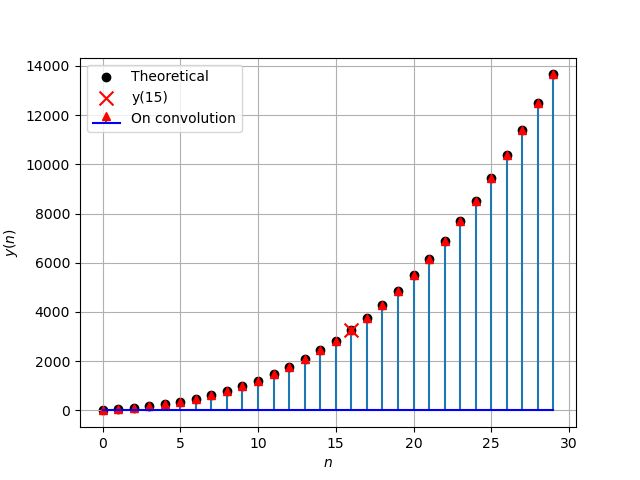
\includegraphics[width=\columnwidth]{ncert-maths/11/9/4/5/figs/plot.png}

\begin{center}
    \caption{Simulation v/s theoretical}
\end{center}
\end{figure}


\pagebreak

\item
The sum of the $4$th and $8$th terms of an AP is $24$ and the sum of the $6$th and $10$th terms is $44$. Find the first three terms of the AP.\\
\solution
 \iffalse
\let\negmedspace\undefined
\let\negthickspace\undefined
\documentclass[journal,12pt,twocolumn]{IEEEtran}
\usepackage{amssymb}
\usepackage{cite}
\usepackage{amsmath,amssymb,amsfonts,amsthm}
\usepackage{algorithmic}
\usepackage{graphicx}
\usepackage{textcomp}
\usepackage{xcolor}
\usepackage{txfonts}
\usepackage{listings}
\usepackage{enumitem}
\usepackage{mathtools}
\usepackage{gensymb}
\usepackage{comment}
\usepackage[breaklinks=true]{hyperref}
\usepackage{tkz-euclide} 
\usepackage{listings}
\usepackage{gvv}                                        
\def\inputGnumericTable{}                                 
\usepackage[latin1]{inputenc}                                
\usepackage{color}                                            
\usepackage{array}                                            
\usepackage{longtable}                                       
\usepackage{calc}                                             
\usepackage{multirow}                                         
\usepackage{hhline}                                           
\usepackage{ifthen}                                           
\usepackage{lscape}
\usepackage{pgfplots}
\newtheorem{theorem}{Theorem}[section]
\newtheorem{problem}{Problem}
\newtheorem{proposition}{Proposition}[section]
\newtheorem{lemma}{Lemma}[section]
\newtheorem{corollary}[theorem]{Corollary}
\newtheorem{example}{Example}[section]
\newtheorem{definition}[problem]{Definition}
\newcommand{\BEQA}{\begin{eqnarray}}
\newcommand{\EEQA}{\end{eqnarray}}
\newcommand{\define}{\stackrel{\triangle}{=}}
\theoremstyle{remark}
\newtheorem{rem}{Remark}
\begin{document}

\bibliographystyle{IEEEtran}
\vspace{3cm}

\title{NCERT Discrete-11.9.4-5}
\author{EE22BTECH11004 - Allu Lohith}

\maketitle
\newpage
\bigskip


 Find the sum of n terms of this sequence:$$5^2+6^2+7^2...+20^2$$  
\solution
\fi
\begin{table}[h!]
\centering
\renewcommand{\arraystretch}{2}
\begin{tabular}{|c|p{4cm}|c|}
\hline 
\setlength{\tabcolsep}{1pt}
\textbf{Parameter}  &\textbf{Description} &\textbf{Formulae/Value} \\
\hline
n & Iteration number starting from zero till 15 & - \\
\hline
$x\brak n$ & General term of the sequence from $n=0$ to $n=15$ &$\brak{n+5}^2$  u\brak n\\
\hline
$x\brak 0$ & First term of the sequence & 5 \\
\hline
\end{tabular}

\vspace{0.5cm}
\caption{\normalsize Parameters}
\end{table}
The standard $z$ transforms,
\begin{align}
    u \brak n &\stackrel{z}{\longleftrightarrow} \frac{1}{1-z^{-1}}, \abs z >1\\
   n u\brak n &\stackrel{z}{\longleftrightarrow} \frac{z^{-1}}{\brak{1-z^{-1}}^2}, \abs z >1\\
   n^2 u\brak n &\stackrel{z}{\longleftrightarrow} \frac{z^{-1}\brak{1+z^{-1}}}{\brak{1-z^{-1}}^3}, \abs z >1
\end{align}
As 
\begin{align}
    x\brak n = \brak{n^2+10n+25}u\brak n
\end{align}
The $z$ transform of general term can be written as , 
\begin{align}
    X\brak z &= \frac{z^{-1}\brak{1+z^{-1}}}{\brak{1-z^{-1}}^3}+10\frac{z^{-1}}{\brak{1-z^{-1}}^2}+\frac{25}{1-z^{-1}} \\
    X\brak z &=  \frac{16z^{-2}-39z^{-1}+25}{\brak{1-z^{-1}}^3}; \abs{z}>1
\end{align}
On convolution for finding the sum
\begin{align}
    y\brak n= x\brak n \ast u\brak n
\end{align}
On z transform,
\begin{align}
    Y\brak z &= X \brak z \cdot U \brak z\\
    &= \brak{\frac{16z^{-2}-39z^{-1}+25}{\brak{1-z^{-1}})^3}} \cdot \frac{1}{1-z^{-1}}\\
    \implies 
    Y \brak z & = \frac{16z^{-2}-39z^{-1}+25}{\brak{1-z^{-1}}^4}; \quad \abs z >1
\end{align}
Using the contour integration to find the inverse $z$ transform,
\begin{align}
    y(n)&=\oint_c Y(z)\cdot z^{n-1}dz\\
    y(21)&=\oint_c \brak{\frac{16z^{-2}-39z^{-1}+25}{\brak{1-z^{-1}}^4}} z^{14}dz
\end{align}
As there are four poles from observation, so $m=4$
\begin{align}
    y\brak{21} &= \frac{1}{(m-1)!} \lim_{z \to a} \frac{d^{m-1}}{dz^{m-1}}\brak{(z-a)^mf(z)}\\
    &= \frac{1}{3!} \lim_{z \to 1} \frac{d^{3}}{dz^{3}}\brak{(z-1)^4 \frac{\brak{16z^{-2}-39z^{-1}+25}}{(1-z^{-1})^4} z^{14}}\\
    &= \frac{1}{6} \lim_{z \to 1} \frac{d^{3}}{dz^{3}}\brak{\brak{16z^{-2}-39z^{-1}+25}z^{18}}\\
    &= \frac{1}{6} \lim_{z \to 1} \frac{d^{3}}{dz^{3}}\brak{16z^{16}-39z^{17}+25z^{18}}\\
    &= \frac{1}{6}  \brak{16 \times 18 \times 17 \times 16+14 \times 17 \times 16 \times 15 }\\
    \implies y\brak{21}&=2840 
\end{align}
Hence the sum of the terms of the sequence is 2840.

\begin{figure}[h]
    \centering  

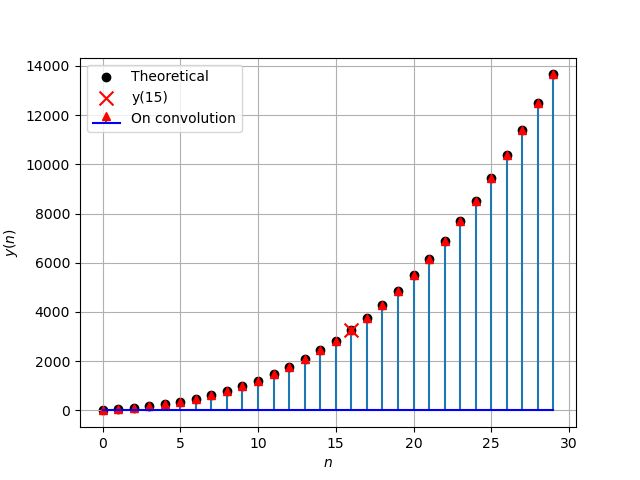
\includegraphics[width=\columnwidth]{ncert-maths/11/9/4/5/figs/plot.png}

\begin{center}
    \caption{Simulation v/s theoretical}
\end{center}
\end{figure}


\newpage

\item
If A and G be A.M. and G.M., respectively between two positive numbers, prove that the numbers are $A \pm \sqrt{(A+G)(A-G)}$\\
\solution
\newpage

 \item
A man starts repaying a loan as first instalment of Rs.$100$. If he increases the
instalment by Rs $5$ every month, what amount he will pay in the $30^{th}$ instalment? \\
\solution
 \iffalse
\let\negmedspace\undefined
\let\negthickspace\undefined
\documentclass[journal,12pt,twocolumn]{IEEEtran}
\usepackage{amssymb}
\usepackage{cite}
\usepackage{amsmath,amssymb,amsfonts,amsthm}
\usepackage{algorithmic}
\usepackage{graphicx}
\usepackage{textcomp}
\usepackage{xcolor}
\usepackage{txfonts}
\usepackage{listings}
\usepackage{enumitem}
\usepackage{mathtools}
\usepackage{gensymb}
\usepackage{comment}
\usepackage[breaklinks=true]{hyperref}
\usepackage{tkz-euclide} 
\usepackage{listings}
\usepackage{gvv}                                        
\def\inputGnumericTable{}                                 
\usepackage[latin1]{inputenc}                                
\usepackage{color}                                            
\usepackage{array}                                            
\usepackage{longtable}                                       
\usepackage{calc}                                             
\usepackage{multirow}                                         
\usepackage{hhline}                                           
\usepackage{ifthen}                                           
\usepackage{lscape}
\usepackage{pgfplots}
\newtheorem{theorem}{Theorem}[section]
\newtheorem{problem}{Problem}
\newtheorem{proposition}{Proposition}[section]
\newtheorem{lemma}{Lemma}[section]
\newtheorem{corollary}[theorem]{Corollary}
\newtheorem{example}{Example}[section]
\newtheorem{definition}[problem]{Definition}
\newcommand{\BEQA}{\begin{eqnarray}}
\newcommand{\EEQA}{\end{eqnarray}}
\newcommand{\define}{\stackrel{\triangle}{=}}
\theoremstyle{remark}
\newtheorem{rem}{Remark}
\begin{document}

\bibliographystyle{IEEEtran}
\vspace{3cm}

\title{NCERT Discrete-11.9.4-5}
\author{EE22BTECH11004 - Allu Lohith}

\maketitle
\newpage
\bigskip


 Find the sum of n terms of this sequence:$$5^2+6^2+7^2...+20^2$$  
\solution
\fi
\begin{table}[h!]
\centering
\renewcommand{\arraystretch}{2}
\begin{tabular}{|c|p{4cm}|c|}
\hline 
\setlength{\tabcolsep}{1pt}
\textbf{Parameter}  &\textbf{Description} &\textbf{Formulae/Value} \\
\hline
n & Iteration number starting from zero till 15 & - \\
\hline
$x\brak n$ & General term of the sequence from $n=0$ to $n=15$ &$\brak{n+5}^2$  u\brak n\\
\hline
$x\brak 0$ & First term of the sequence & 5 \\
\hline
\end{tabular}

\vspace{0.5cm}
\caption{\normalsize Parameters}
\end{table}
The standard $z$ transforms,
\begin{align}
    u \brak n &\stackrel{z}{\longleftrightarrow} \frac{1}{1-z^{-1}}, \abs z >1\\
   n u\brak n &\stackrel{z}{\longleftrightarrow} \frac{z^{-1}}{\brak{1-z^{-1}}^2}, \abs z >1\\
   n^2 u\brak n &\stackrel{z}{\longleftrightarrow} \frac{z^{-1}\brak{1+z^{-1}}}{\brak{1-z^{-1}}^3}, \abs z >1
\end{align}
As 
\begin{align}
    x\brak n = \brak{n^2+10n+25}u\brak n
\end{align}
The $z$ transform of general term can be written as , 
\begin{align}
    X\brak z &= \frac{z^{-1}\brak{1+z^{-1}}}{\brak{1-z^{-1}}^3}+10\frac{z^{-1}}{\brak{1-z^{-1}}^2}+\frac{25}{1-z^{-1}} \\
    X\brak z &=  \frac{16z^{-2}-39z^{-1}+25}{\brak{1-z^{-1}}^3}; \abs{z}>1
\end{align}
On convolution for finding the sum
\begin{align}
    y\brak n= x\brak n \ast u\brak n
\end{align}
On z transform,
\begin{align}
    Y\brak z &= X \brak z \cdot U \brak z\\
    &= \brak{\frac{16z^{-2}-39z^{-1}+25}{\brak{1-z^{-1}})^3}} \cdot \frac{1}{1-z^{-1}}\\
    \implies 
    Y \brak z & = \frac{16z^{-2}-39z^{-1}+25}{\brak{1-z^{-1}}^4}; \quad \abs z >1
\end{align}
Using the contour integration to find the inverse $z$ transform,
\begin{align}
    y(n)&=\oint_c Y(z)\cdot z^{n-1}dz\\
    y(21)&=\oint_c \brak{\frac{16z^{-2}-39z^{-1}+25}{\brak{1-z^{-1}}^4}} z^{14}dz
\end{align}
As there are four poles from observation, so $m=4$
\begin{align}
    y\brak{21} &= \frac{1}{(m-1)!} \lim_{z \to a} \frac{d^{m-1}}{dz^{m-1}}\brak{(z-a)^mf(z)}\\
    &= \frac{1}{3!} \lim_{z \to 1} \frac{d^{3}}{dz^{3}}\brak{(z-1)^4 \frac{\brak{16z^{-2}-39z^{-1}+25}}{(1-z^{-1})^4} z^{14}}\\
    &= \frac{1}{6} \lim_{z \to 1} \frac{d^{3}}{dz^{3}}\brak{\brak{16z^{-2}-39z^{-1}+25}z^{18}}\\
    &= \frac{1}{6} \lim_{z \to 1} \frac{d^{3}}{dz^{3}}\brak{16z^{16}-39z^{17}+25z^{18}}\\
    &= \frac{1}{6}  \brak{16 \times 18 \times 17 \times 16+14 \times 17 \times 16 \times 15 }\\
    \implies y\brak{21}&=2840 
\end{align}
Hence the sum of the terms of the sequence is 2840.

\begin{figure}[h]
    \centering  

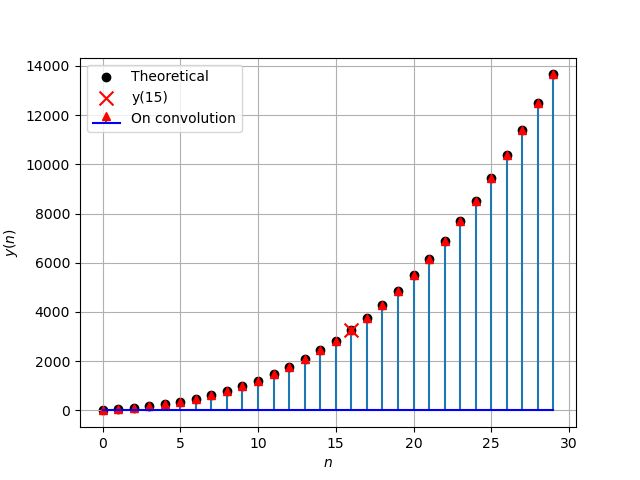
\includegraphics[width=\columnwidth]{ncert-maths/11/9/4/5/figs/plot.png}

\begin{center}
    \caption{Simulation v/s theoretical}
\end{center}
\end{figure}


\newpage

\item 
Write the first five terms of the sequence $a_n = n(n+2)$. \\
\solution
\input{ncert-maths/11/9/1/1/d124.tex}
\newpage
\item If A.M. and G.M. of roots of a quadratic equation are 8 and 5,respectively,then obtain the quadratic equation.
\solution
\input{ncert-maths/11/9/3/32/32.tex}
\pagebreak

\item An AP consists of $50$ terms of which $3^{rd}$ term is $12$ and the last term is $106$. Find the $29^{th}$ term.\\
\solution 
\input{ncert-maths/10/5/2/8/problem1.tex}
\pagebreak

\item The first term of an AP is $5$, the last term is $45$ and the sum is $400$. Find the number of terms and the common difference.\\
\solution
 \iffalse
\let\negmedspace\undefined
\let\negthickspace\undefined
\documentclass[journal,12pt,twocolumn]{IEEEtran}
\usepackage{amssymb}
\usepackage{cite}
\usepackage{amsmath,amssymb,amsfonts,amsthm}
\usepackage{algorithmic}
\usepackage{graphicx}
\usepackage{textcomp}
\usepackage{xcolor}
\usepackage{txfonts}
\usepackage{listings}
\usepackage{enumitem}
\usepackage{mathtools}
\usepackage{gensymb}
\usepackage{comment}
\usepackage[breaklinks=true]{hyperref}
\usepackage{tkz-euclide} 
\usepackage{listings}
\usepackage{gvv}                                        
\def\inputGnumericTable{}                                 
\usepackage[latin1]{inputenc}                                
\usepackage{color}                                            
\usepackage{array}                                            
\usepackage{longtable}                                       
\usepackage{calc}                                             
\usepackage{multirow}                                         
\usepackage{hhline}                                           
\usepackage{ifthen}                                           
\usepackage{lscape}
\usepackage{pgfplots}
\newtheorem{theorem}{Theorem}[section]
\newtheorem{problem}{Problem}
\newtheorem{proposition}{Proposition}[section]
\newtheorem{lemma}{Lemma}[section]
\newtheorem{corollary}[theorem]{Corollary}
\newtheorem{example}{Example}[section]
\newtheorem{definition}[problem]{Definition}
\newcommand{\BEQA}{\begin{eqnarray}}
\newcommand{\EEQA}{\end{eqnarray}}
\newcommand{\define}{\stackrel{\triangle}{=}}
\theoremstyle{remark}
\newtheorem{rem}{Remark}
\begin{document}

\bibliographystyle{IEEEtran}
\vspace{3cm}

\title{NCERT Discrete-11.9.4-5}
\author{EE22BTECH11004 - Allu Lohith}

\maketitle
\newpage
\bigskip


 Find the sum of n terms of this sequence:$$5^2+6^2+7^2...+20^2$$  
\solution
\fi
\begin{table}[h!]
\centering
\renewcommand{\arraystretch}{2}
\begin{tabular}{|c|p{4cm}|c|}
\hline 
\setlength{\tabcolsep}{1pt}
\textbf{Parameter}  &\textbf{Description} &\textbf{Formulae/Value} \\
\hline
n & Iteration number starting from zero till 15 & - \\
\hline
$x\brak n$ & General term of the sequence from $n=0$ to $n=15$ &$\brak{n+5}^2$  u\brak n\\
\hline
$x\brak 0$ & First term of the sequence & 5 \\
\hline
\end{tabular}

\vspace{0.5cm}
\caption{\normalsize Parameters}
\end{table}
The standard $z$ transforms,
\begin{align}
    u \brak n &\stackrel{z}{\longleftrightarrow} \frac{1}{1-z^{-1}}, \abs z >1\\
   n u\brak n &\stackrel{z}{\longleftrightarrow} \frac{z^{-1}}{\brak{1-z^{-1}}^2}, \abs z >1\\
   n^2 u\brak n &\stackrel{z}{\longleftrightarrow} \frac{z^{-1}\brak{1+z^{-1}}}{\brak{1-z^{-1}}^3}, \abs z >1
\end{align}
As 
\begin{align}
    x\brak n = \brak{n^2+10n+25}u\brak n
\end{align}
The $z$ transform of general term can be written as , 
\begin{align}
    X\brak z &= \frac{z^{-1}\brak{1+z^{-1}}}{\brak{1-z^{-1}}^3}+10\frac{z^{-1}}{\brak{1-z^{-1}}^2}+\frac{25}{1-z^{-1}} \\
    X\brak z &=  \frac{16z^{-2}-39z^{-1}+25}{\brak{1-z^{-1}}^3}; \abs{z}>1
\end{align}
On convolution for finding the sum
\begin{align}
    y\brak n= x\brak n \ast u\brak n
\end{align}
On z transform,
\begin{align}
    Y\brak z &= X \brak z \cdot U \brak z\\
    &= \brak{\frac{16z^{-2}-39z^{-1}+25}{\brak{1-z^{-1}})^3}} \cdot \frac{1}{1-z^{-1}}\\
    \implies 
    Y \brak z & = \frac{16z^{-2}-39z^{-1}+25}{\brak{1-z^{-1}}^4}; \quad \abs z >1
\end{align}
Using the contour integration to find the inverse $z$ transform,
\begin{align}
    y(n)&=\oint_c Y(z)\cdot z^{n-1}dz\\
    y(21)&=\oint_c \brak{\frac{16z^{-2}-39z^{-1}+25}{\brak{1-z^{-1}}^4}} z^{14}dz
\end{align}
As there are four poles from observation, so $m=4$
\begin{align}
    y\brak{21} &= \frac{1}{(m-1)!} \lim_{z \to a} \frac{d^{m-1}}{dz^{m-1}}\brak{(z-a)^mf(z)}\\
    &= \frac{1}{3!} \lim_{z \to 1} \frac{d^{3}}{dz^{3}}\brak{(z-1)^4 \frac{\brak{16z^{-2}-39z^{-1}+25}}{(1-z^{-1})^4} z^{14}}\\
    &= \frac{1}{6} \lim_{z \to 1} \frac{d^{3}}{dz^{3}}\brak{\brak{16z^{-2}-39z^{-1}+25}z^{18}}\\
    &= \frac{1}{6} \lim_{z \to 1} \frac{d^{3}}{dz^{3}}\brak{16z^{16}-39z^{17}+25z^{18}}\\
    &= \frac{1}{6}  \brak{16 \times 18 \times 17 \times 16+14 \times 17 \times 16 \times 15 }\\
    \implies y\brak{21}&=2840 
\end{align}
Hence the sum of the terms of the sequence is 2840.

\begin{figure}[h]
    \centering  

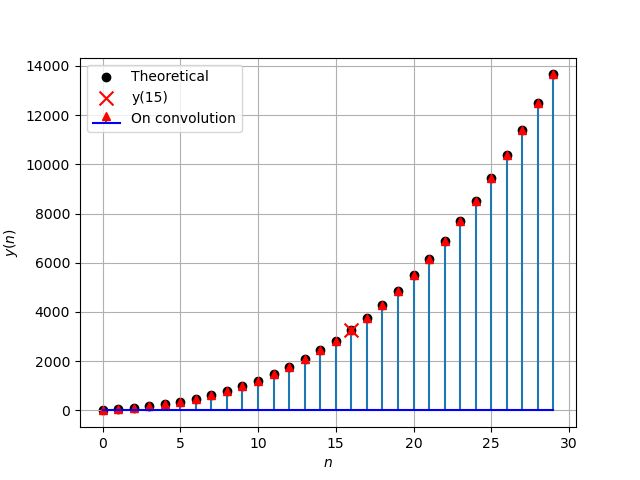
\includegraphics[width=\columnwidth]{ncert-maths/11/9/4/5/figs/plot.png}

\begin{center}
    \caption{Simulation v/s theoretical}
\end{center}
\end{figure}


\pagebreak

\item Which term of the arithmetic progression (AP): \(3, 8, 13, 18, \ldots\) is \(78\)?\\
\solution
\input{ncert-maths/10/5/2/4/ass1.tex}
\pagebreak

\item The sum of two numbers is $6$ times their geometric mean, show that numbers are in the ratio $\dfrac{(3+2\sqrt{2})}{(3-2\sqrt{2})}$. 
\solution
 \iffalse
\let\negmedspace\undefined
\let\negthickspace\undefined
\documentclass[journal,12pt,twocolumn]{IEEEtran}
\usepackage{amssymb}
\usepackage{cite}
\usepackage{amsmath,amssymb,amsfonts,amsthm}
\usepackage{algorithmic}
\usepackage{graphicx}
\usepackage{textcomp}
\usepackage{xcolor}
\usepackage{txfonts}
\usepackage{listings}
\usepackage{enumitem}
\usepackage{mathtools}
\usepackage{gensymb}
\usepackage{comment}
\usepackage[breaklinks=true]{hyperref}
\usepackage{tkz-euclide} 
\usepackage{listings}
\usepackage{gvv}                                        
\def\inputGnumericTable{}                                 
\usepackage[latin1]{inputenc}                                
\usepackage{color}                                            
\usepackage{array}                                            
\usepackage{longtable}                                       
\usepackage{calc}                                             
\usepackage{multirow}                                         
\usepackage{hhline}                                           
\usepackage{ifthen}                                           
\usepackage{lscape}
\usepackage{pgfplots}
\newtheorem{theorem}{Theorem}[section]
\newtheorem{problem}{Problem}
\newtheorem{proposition}{Proposition}[section]
\newtheorem{lemma}{Lemma}[section]
\newtheorem{corollary}[theorem]{Corollary}
\newtheorem{example}{Example}[section]
\newtheorem{definition}[problem]{Definition}
\newcommand{\BEQA}{\begin{eqnarray}}
\newcommand{\EEQA}{\end{eqnarray}}
\newcommand{\define}{\stackrel{\triangle}{=}}
\theoremstyle{remark}
\newtheorem{rem}{Remark}
\begin{document}

\bibliographystyle{IEEEtran}
\vspace{3cm}

\title{NCERT Discrete-11.9.4-5}
\author{EE22BTECH11004 - Allu Lohith}

\maketitle
\newpage
\bigskip


 Find the sum of n terms of this sequence:$$5^2+6^2+7^2...+20^2$$  
\solution
\fi
\begin{table}[h!]
\centering
\renewcommand{\arraystretch}{2}
\begin{tabular}{|c|p{4cm}|c|}
\hline 
\setlength{\tabcolsep}{1pt}
\textbf{Parameter}  &\textbf{Description} &\textbf{Formulae/Value} \\
\hline
n & Iteration number starting from zero till 15 & - \\
\hline
$x\brak n$ & General term of the sequence from $n=0$ to $n=15$ &$\brak{n+5}^2$  u\brak n\\
\hline
$x\brak 0$ & First term of the sequence & 5 \\
\hline
\end{tabular}

\vspace{0.5cm}
\caption{\normalsize Parameters}
\end{table}
The standard $z$ transforms,
\begin{align}
    u \brak n &\stackrel{z}{\longleftrightarrow} \frac{1}{1-z^{-1}}, \abs z >1\\
   n u\brak n &\stackrel{z}{\longleftrightarrow} \frac{z^{-1}}{\brak{1-z^{-1}}^2}, \abs z >1\\
   n^2 u\brak n &\stackrel{z}{\longleftrightarrow} \frac{z^{-1}\brak{1+z^{-1}}}{\brak{1-z^{-1}}^3}, \abs z >1
\end{align}
As 
\begin{align}
    x\brak n = \brak{n^2+10n+25}u\brak n
\end{align}
The $z$ transform of general term can be written as , 
\begin{align}
    X\brak z &= \frac{z^{-1}\brak{1+z^{-1}}}{\brak{1-z^{-1}}^3}+10\frac{z^{-1}}{\brak{1-z^{-1}}^2}+\frac{25}{1-z^{-1}} \\
    X\brak z &=  \frac{16z^{-2}-39z^{-1}+25}{\brak{1-z^{-1}}^3}; \abs{z}>1
\end{align}
On convolution for finding the sum
\begin{align}
    y\brak n= x\brak n \ast u\brak n
\end{align}
On z transform,
\begin{align}
    Y\brak z &= X \brak z \cdot U \brak z\\
    &= \brak{\frac{16z^{-2}-39z^{-1}+25}{\brak{1-z^{-1}})^3}} \cdot \frac{1}{1-z^{-1}}\\
    \implies 
    Y \brak z & = \frac{16z^{-2}-39z^{-1}+25}{\brak{1-z^{-1}}^4}; \quad \abs z >1
\end{align}
Using the contour integration to find the inverse $z$ transform,
\begin{align}
    y(n)&=\oint_c Y(z)\cdot z^{n-1}dz\\
    y(21)&=\oint_c \brak{\frac{16z^{-2}-39z^{-1}+25}{\brak{1-z^{-1}}^4}} z^{14}dz
\end{align}
As there are four poles from observation, so $m=4$
\begin{align}
    y\brak{21} &= \frac{1}{(m-1)!} \lim_{z \to a} \frac{d^{m-1}}{dz^{m-1}}\brak{(z-a)^mf(z)}\\
    &= \frac{1}{3!} \lim_{z \to 1} \frac{d^{3}}{dz^{3}}\brak{(z-1)^4 \frac{\brak{16z^{-2}-39z^{-1}+25}}{(1-z^{-1})^4} z^{14}}\\
    &= \frac{1}{6} \lim_{z \to 1} \frac{d^{3}}{dz^{3}}\brak{\brak{16z^{-2}-39z^{-1}+25}z^{18}}\\
    &= \frac{1}{6} \lim_{z \to 1} \frac{d^{3}}{dz^{3}}\brak{16z^{16}-39z^{17}+25z^{18}}\\
    &= \frac{1}{6}  \brak{16 \times 18 \times 17 \times 16+14 \times 17 \times 16 \times 15 }\\
    \implies y\brak{21}&=2840 
\end{align}
Hence the sum of the terms of the sequence is 2840.

\begin{figure}[h]
    \centering  

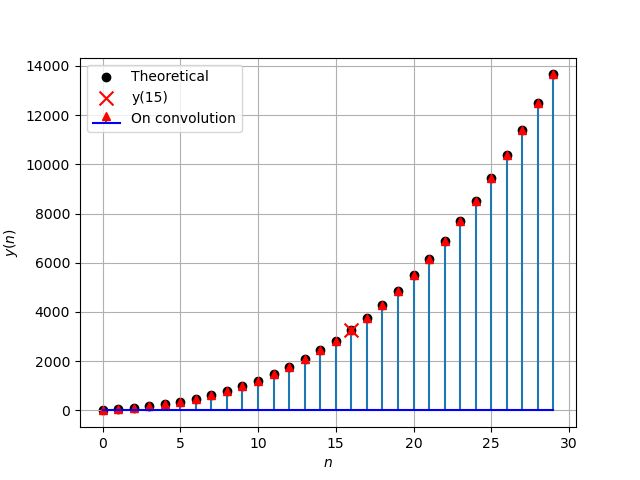
\includegraphics[width=\columnwidth]{ncert-maths/11/9/4/5/figs/plot.png}

\begin{center}
    \caption{Simulation v/s theoretical}
\end{center}
\end{figure}


\pagebreak

\item Find the value of $n$ so that $\frac{a^{n+1} + b^{n+1}}{a^{n}+b^{n}}$ may be the geometric mean between $a$ and $b$. \\
\solution
\input{ncert-maths/11/9/3/27/2.tex}
\pagebreak

\item Which term of the AP : 121, 117, 113, \ldots, is its first negative term?\\
\solution
\pagebreak

\item The first term of a G.P. is $1$. The sum of the third term and fifth term is $90$. Find the common ratio of G.P.\\
\solution
\pagebreak

\item If the sum of first $p$ terms of an A.P. is equal to the sum of the first $q$ terms, then find the sum of the first $(p + q)$ terms.\\
\solution
\pagebreak
\item How many terms of G.P.$3$,$3^2$,$3^3$, \ldots are needed to give the sum $120$ ?\\
\solution
\input{ncert-maths/11/9/3/13/a1.tex}
\pagebreak

\item Find the sum of first $51$ terms of an $AP$ whose second and third terms are $14$ and $18$ respectively. \\
\solution
 \iffalse
\let\negmedspace\undefined
\let\negthickspace\undefined
\documentclass[journal,12pt,twocolumn]{IEEEtran}
\usepackage{amssymb}
\usepackage{cite}
\usepackage{amsmath,amssymb,amsfonts,amsthm}
\usepackage{algorithmic}
\usepackage{graphicx}
\usepackage{textcomp}
\usepackage{xcolor}
\usepackage{txfonts}
\usepackage{listings}
\usepackage{enumitem}
\usepackage{mathtools}
\usepackage{gensymb}
\usepackage{comment}
\usepackage[breaklinks=true]{hyperref}
\usepackage{tkz-euclide} 
\usepackage{listings}
\usepackage{gvv}                                        
\def\inputGnumericTable{}                                 
\usepackage[latin1]{inputenc}                                
\usepackage{color}                                            
\usepackage{array}                                            
\usepackage{longtable}                                       
\usepackage{calc}                                             
\usepackage{multirow}                                         
\usepackage{hhline}                                           
\usepackage{ifthen}                                           
\usepackage{lscape}
\usepackage{pgfplots}
\newtheorem{theorem}{Theorem}[section]
\newtheorem{problem}{Problem}
\newtheorem{proposition}{Proposition}[section]
\newtheorem{lemma}{Lemma}[section]
\newtheorem{corollary}[theorem]{Corollary}
\newtheorem{example}{Example}[section]
\newtheorem{definition}[problem]{Definition}
\newcommand{\BEQA}{\begin{eqnarray}}
\newcommand{\EEQA}{\end{eqnarray}}
\newcommand{\define}{\stackrel{\triangle}{=}}
\theoremstyle{remark}
\newtheorem{rem}{Remark}
\begin{document}

\bibliographystyle{IEEEtran}
\vspace{3cm}

\title{NCERT Discrete-11.9.4-5}
\author{EE22BTECH11004 - Allu Lohith}

\maketitle
\newpage
\bigskip


 Find the sum of n terms of this sequence:$$5^2+6^2+7^2...+20^2$$  
\solution
\fi
\begin{table}[h!]
\centering
\renewcommand{\arraystretch}{2}
\begin{tabular}{|c|p{4cm}|c|}
\hline 
\setlength{\tabcolsep}{1pt}
\textbf{Parameter}  &\textbf{Description} &\textbf{Formulae/Value} \\
\hline
n & Iteration number starting from zero till 15 & - \\
\hline
$x\brak n$ & General term of the sequence from $n=0$ to $n=15$ &$\brak{n+5}^2$  u\brak n\\
\hline
$x\brak 0$ & First term of the sequence & 5 \\
\hline
\end{tabular}

\vspace{0.5cm}
\caption{\normalsize Parameters}
\end{table}
The standard $z$ transforms,
\begin{align}
    u \brak n &\stackrel{z}{\longleftrightarrow} \frac{1}{1-z^{-1}}, \abs z >1\\
   n u\brak n &\stackrel{z}{\longleftrightarrow} \frac{z^{-1}}{\brak{1-z^{-1}}^2}, \abs z >1\\
   n^2 u\brak n &\stackrel{z}{\longleftrightarrow} \frac{z^{-1}\brak{1+z^{-1}}}{\brak{1-z^{-1}}^3}, \abs z >1
\end{align}
As 
\begin{align}
    x\brak n = \brak{n^2+10n+25}u\brak n
\end{align}
The $z$ transform of general term can be written as , 
\begin{align}
    X\brak z &= \frac{z^{-1}\brak{1+z^{-1}}}{\brak{1-z^{-1}}^3}+10\frac{z^{-1}}{\brak{1-z^{-1}}^2}+\frac{25}{1-z^{-1}} \\
    X\brak z &=  \frac{16z^{-2}-39z^{-1}+25}{\brak{1-z^{-1}}^3}; \abs{z}>1
\end{align}
On convolution for finding the sum
\begin{align}
    y\brak n= x\brak n \ast u\brak n
\end{align}
On z transform,
\begin{align}
    Y\brak z &= X \brak z \cdot U \brak z\\
    &= \brak{\frac{16z^{-2}-39z^{-1}+25}{\brak{1-z^{-1}})^3}} \cdot \frac{1}{1-z^{-1}}\\
    \implies 
    Y \brak z & = \frac{16z^{-2}-39z^{-1}+25}{\brak{1-z^{-1}}^4}; \quad \abs z >1
\end{align}
Using the contour integration to find the inverse $z$ transform,
\begin{align}
    y(n)&=\oint_c Y(z)\cdot z^{n-1}dz\\
    y(21)&=\oint_c \brak{\frac{16z^{-2}-39z^{-1}+25}{\brak{1-z^{-1}}^4}} z^{14}dz
\end{align}
As there are four poles from observation, so $m=4$
\begin{align}
    y\brak{21} &= \frac{1}{(m-1)!} \lim_{z \to a} \frac{d^{m-1}}{dz^{m-1}}\brak{(z-a)^mf(z)}\\
    &= \frac{1}{3!} \lim_{z \to 1} \frac{d^{3}}{dz^{3}}\brak{(z-1)^4 \frac{\brak{16z^{-2}-39z^{-1}+25}}{(1-z^{-1})^4} z^{14}}\\
    &= \frac{1}{6} \lim_{z \to 1} \frac{d^{3}}{dz^{3}}\brak{\brak{16z^{-2}-39z^{-1}+25}z^{18}}\\
    &= \frac{1}{6} \lim_{z \to 1} \frac{d^{3}}{dz^{3}}\brak{16z^{16}-39z^{17}+25z^{18}}\\
    &= \frac{1}{6}  \brak{16 \times 18 \times 17 \times 16+14 \times 17 \times 16 \times 15 }\\
    \implies y\brak{21}&=2840 
\end{align}
Hence the sum of the terms of the sequence is 2840.

\begin{figure}[h]
    \centering  

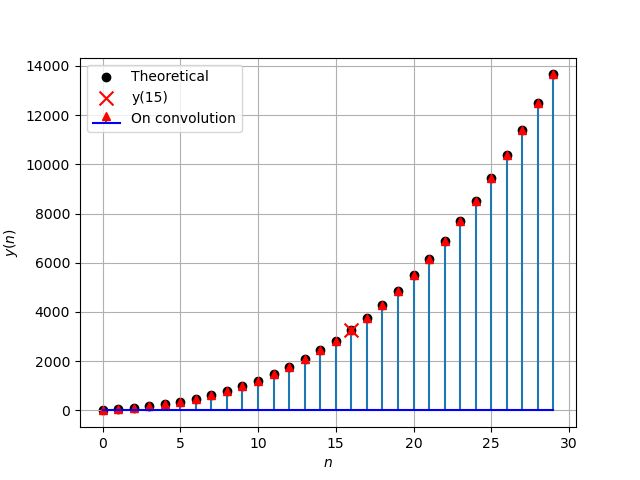
\includegraphics[width=\columnwidth]{ncert-maths/11/9/4/5/figs/plot.png}

\begin{center}
    \caption{Simulation v/s theoretical}
\end{center}
\end{figure}


\pagebreak

\item Fill in the blanks in the following table given that $a$ is the first term, $d$ is the common difference, and $a_n$ is the $n$th term of the AP.\\
\begin{table}[h!]
  \centering
  \input{ncert-maths/10/5/2/1/tables/10.5.2.1.table.tex}
   \label{tab:ESTable1}
\end{table}
\solution
\input{ncert-maths/10/5/2/1/10.tex}
\pagebreak
\end{enumerate}
